\chapter{Spectral ViT Model Performance}
\label{chap:chapter-4}


\section{V1}\label{sec:v1_results}
The Spectral ViT's performance was evaluated on the test set of 12888 validation spectra.
These spectra were not used in the training, nor the test set of the model. The resulting 
ROC curve and confusion matrix are shown in Figure~\ref{fig:v1_qual}. The ROC curve 
shows the model is capable of differentiating between SNe and non-SNe with an AUC of 0.99.
However, differentiating between the different types of SNe is more difficult, as the
confusion matrix indicates. 
\begin{figure}
    \centering
    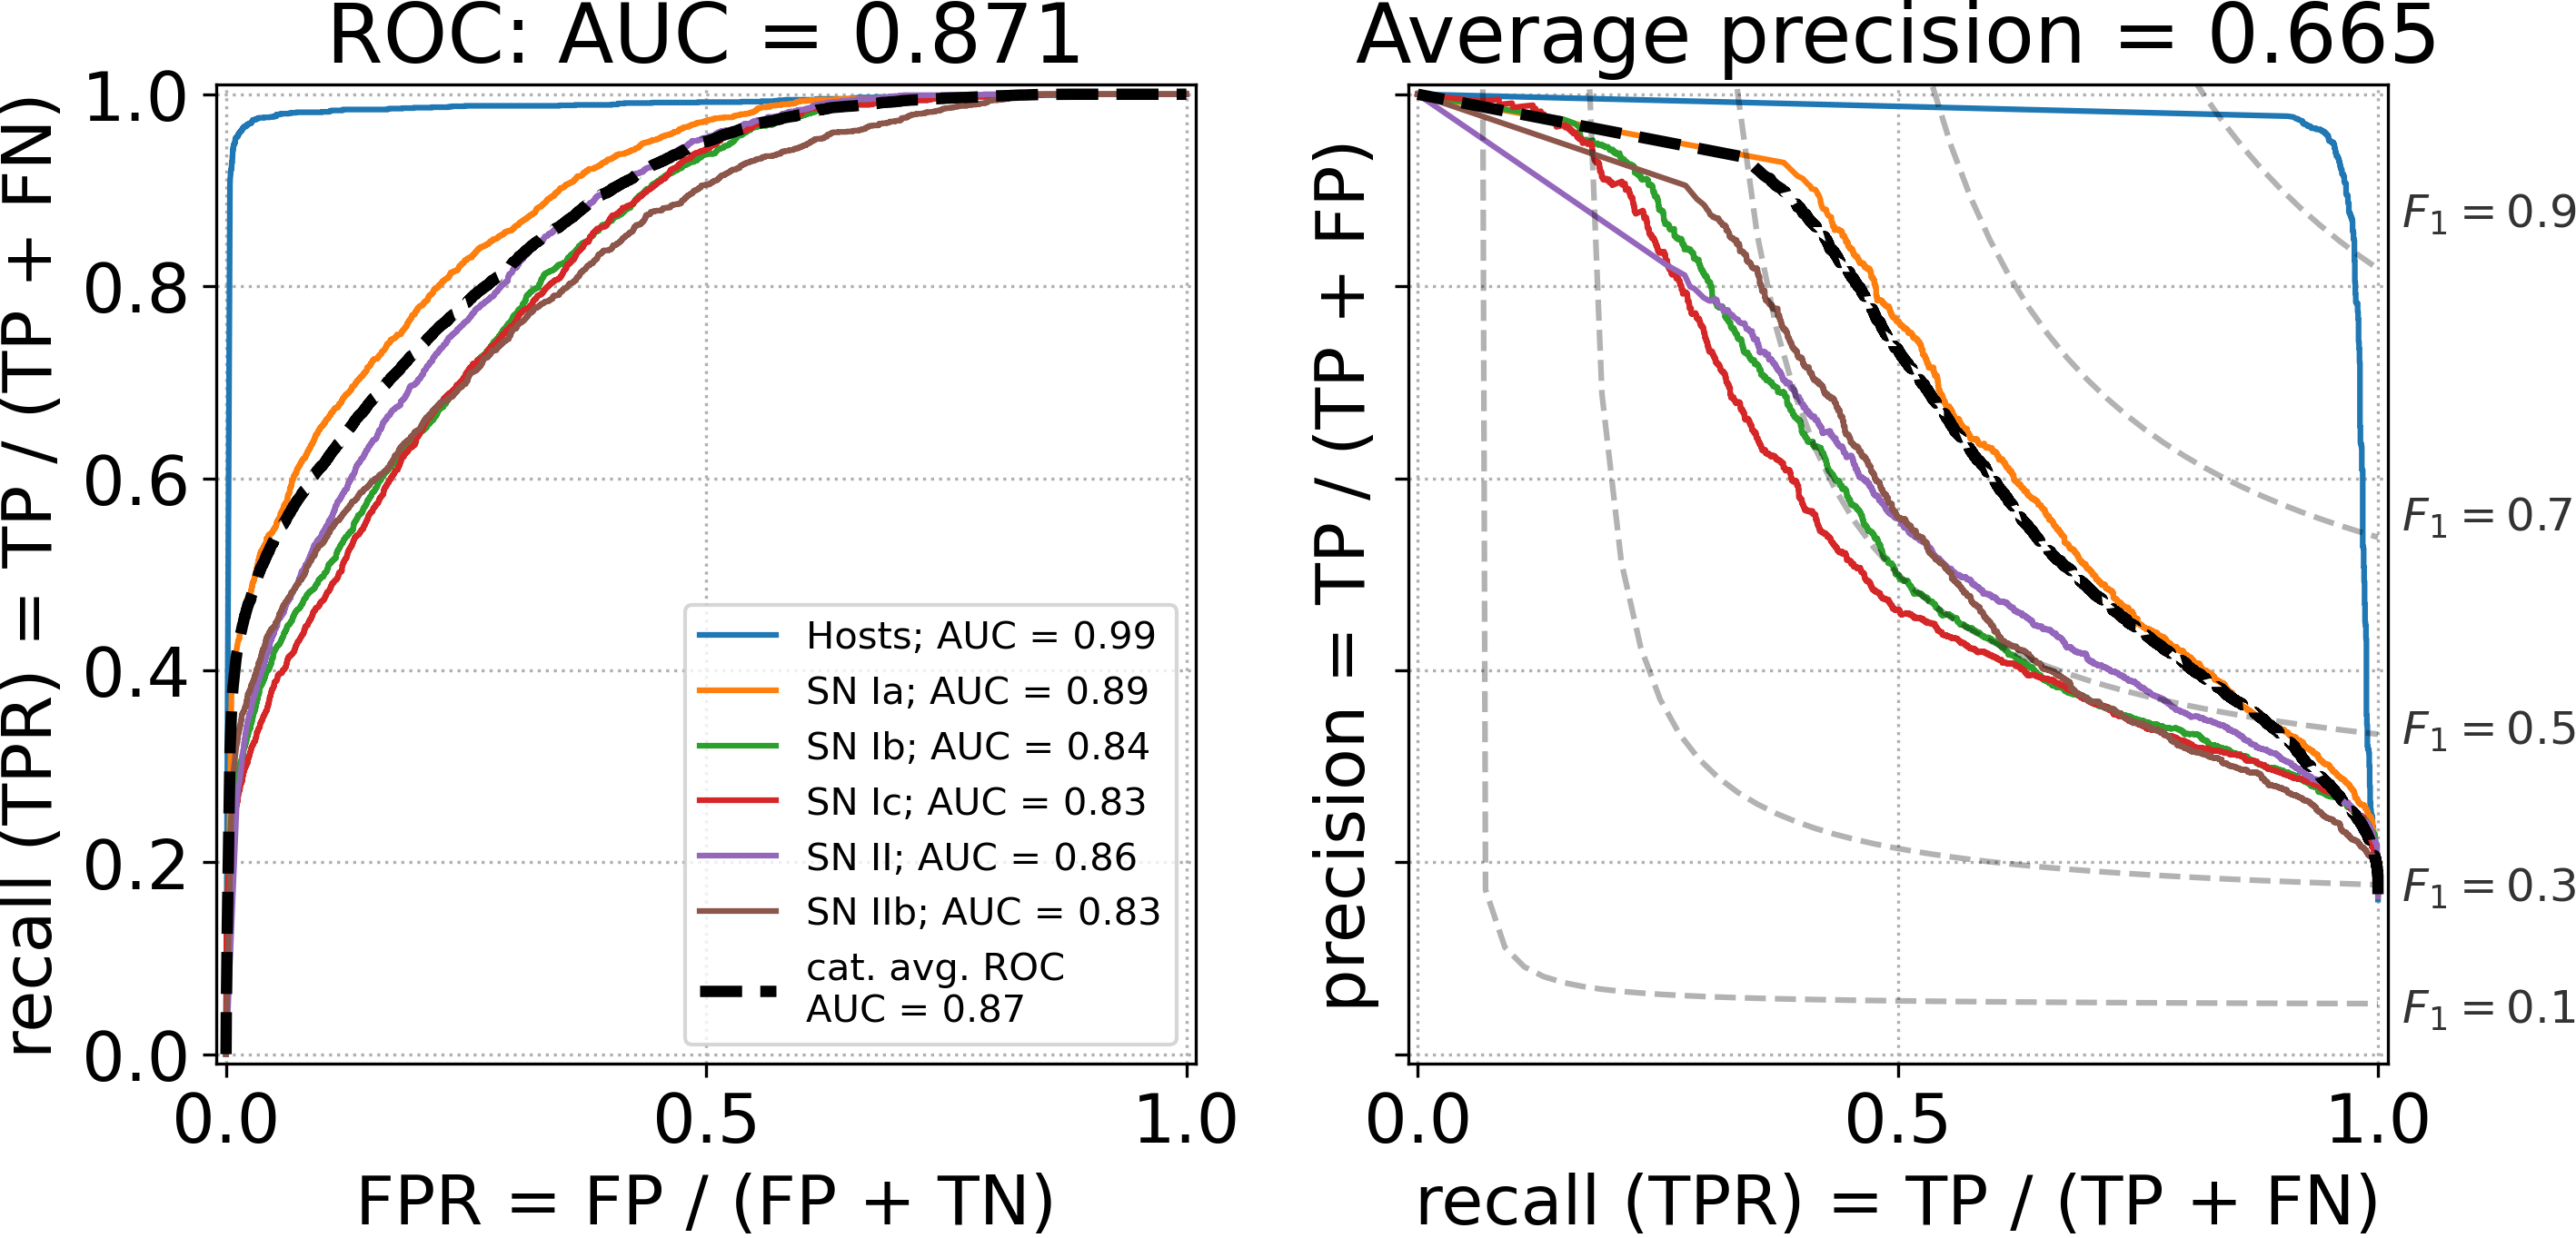
\includegraphics[height=4.3cm]{figures/v1_real/vit_model_V1_original_redorocfulle_e31.png}
    \quad
    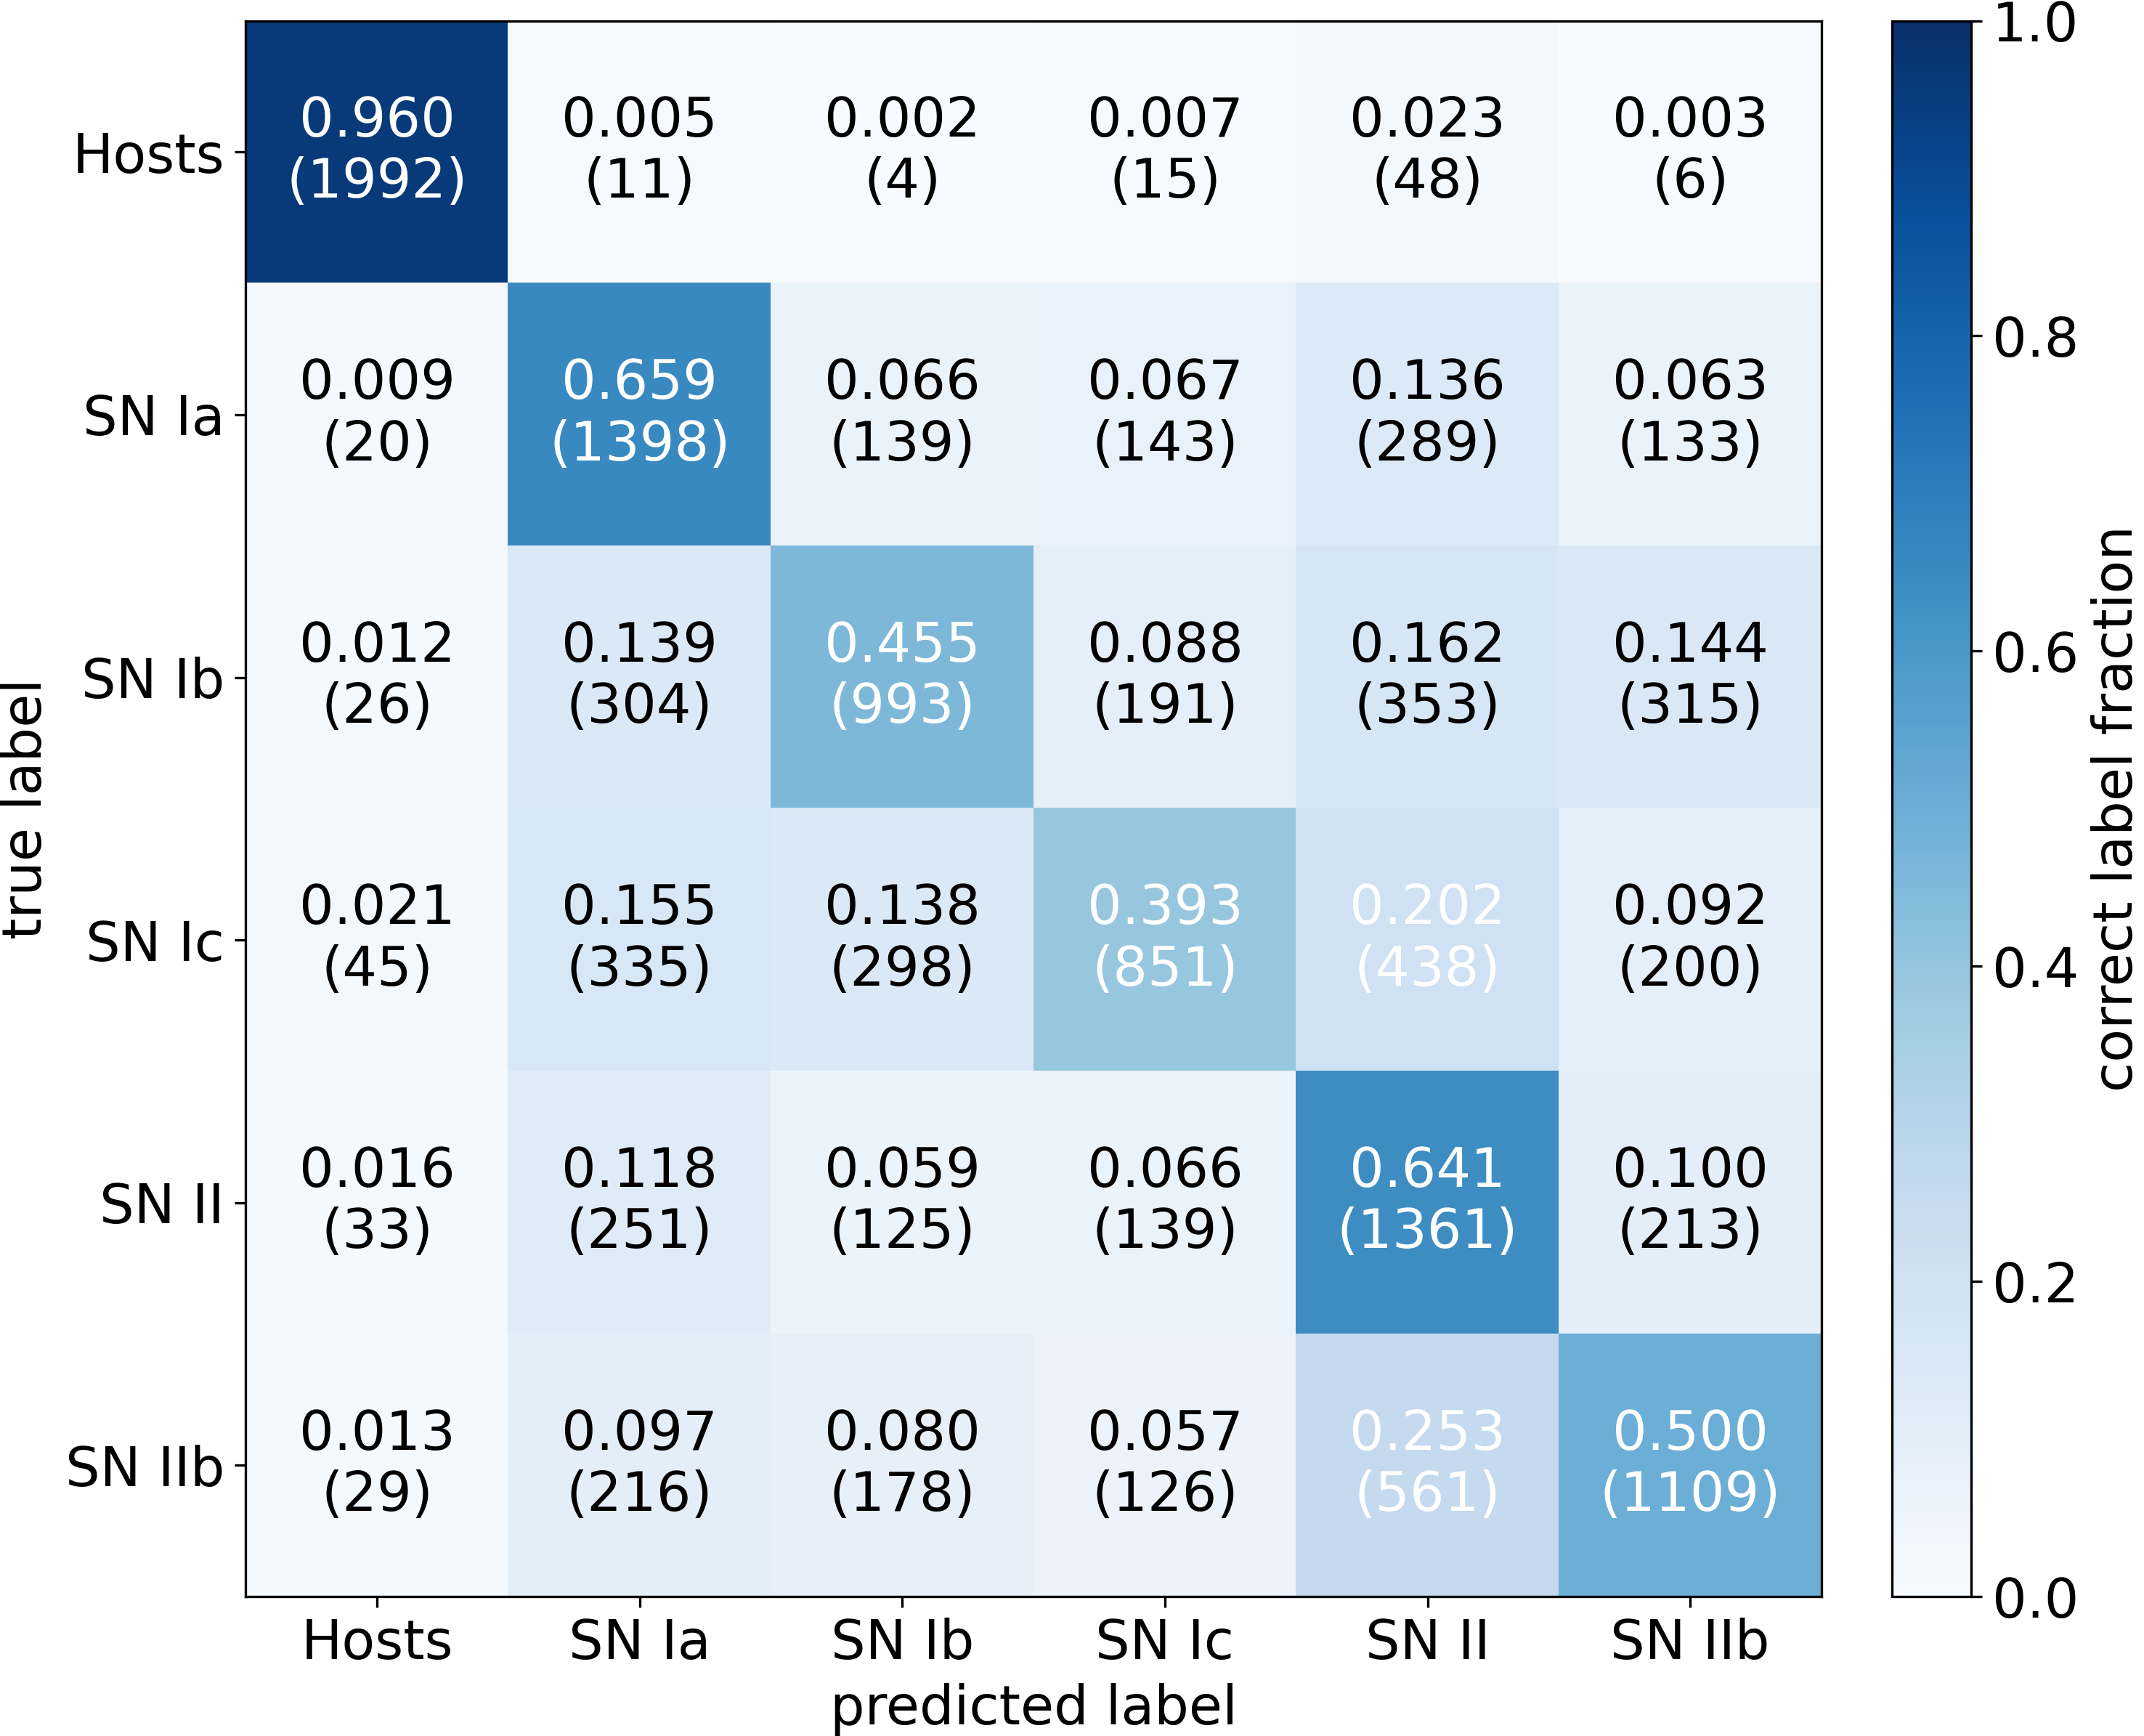
\includegraphics[height=4.3cm]{figures/v1_real/vit_model_V1_original_redocmfull_e31.png}
    \caption{Spectral ViT V1 Diagnostics: ROC Curve (left) and Confusion Matrix (right)\label{fig:v1_qual}}
\end{figure}

In contrast to the CNN previously used by \textcite{Sepeku2022}, the Spectral ViT V1 
was more sure of its predictions, as indicated by Figure~\ref{fig:v1_max}. By filtering 
out predictions with a maximum value less than 99\%, the model's average precision 
was increased from 0.665 to 0.783 (Figure~\ref{fig:v1_99_qual}). This cut included 
63.4\% of the original predictions. Further increasing this cut to 99.9999\% reduced 
the sample size to 5156 (40\% of the original validation size), but further increased the 
average precision to 0.862, as shown in Figure~\ref{fig:v1_999999_qual}.  
\begin{figure}[t]
    \centering
    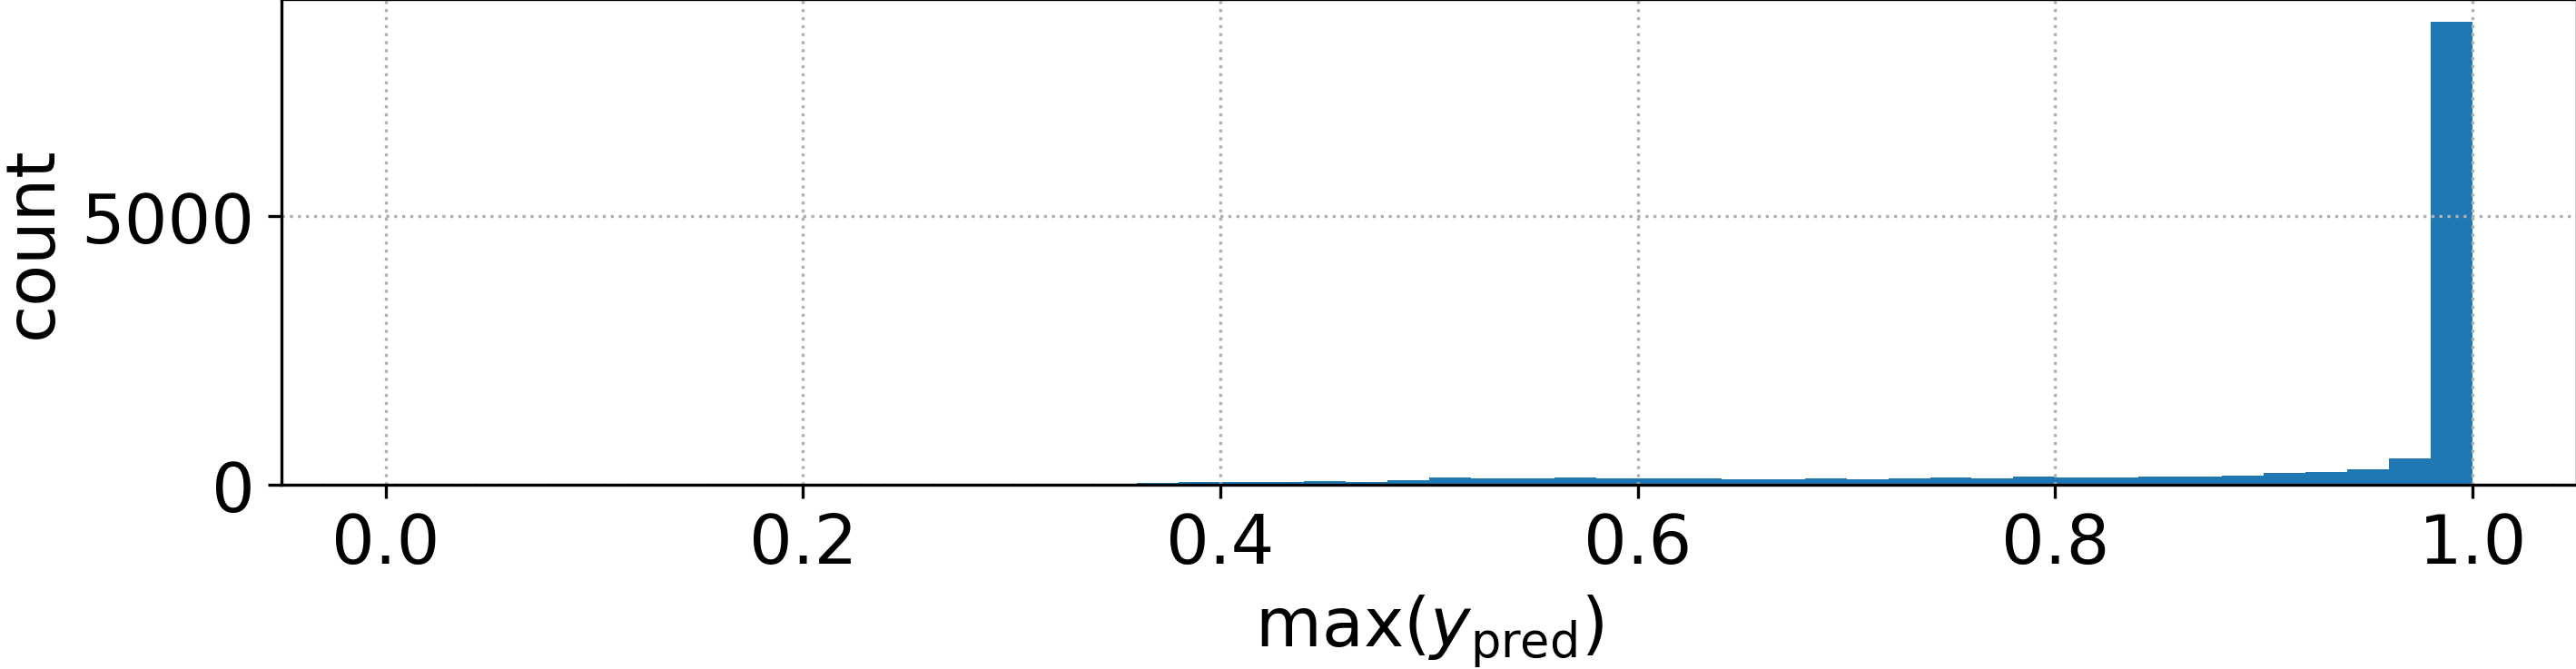
\includegraphics[width=0.6\textwidth]{figures/v1_real/vit_model_V1_original_redomax_ypred_binary_31.png}
    \caption{Max value of the output vector from the Spectral ViT V1.\label{fig:v1_max}}
\end{figure}

\begin{figure}[b]
    \centering
    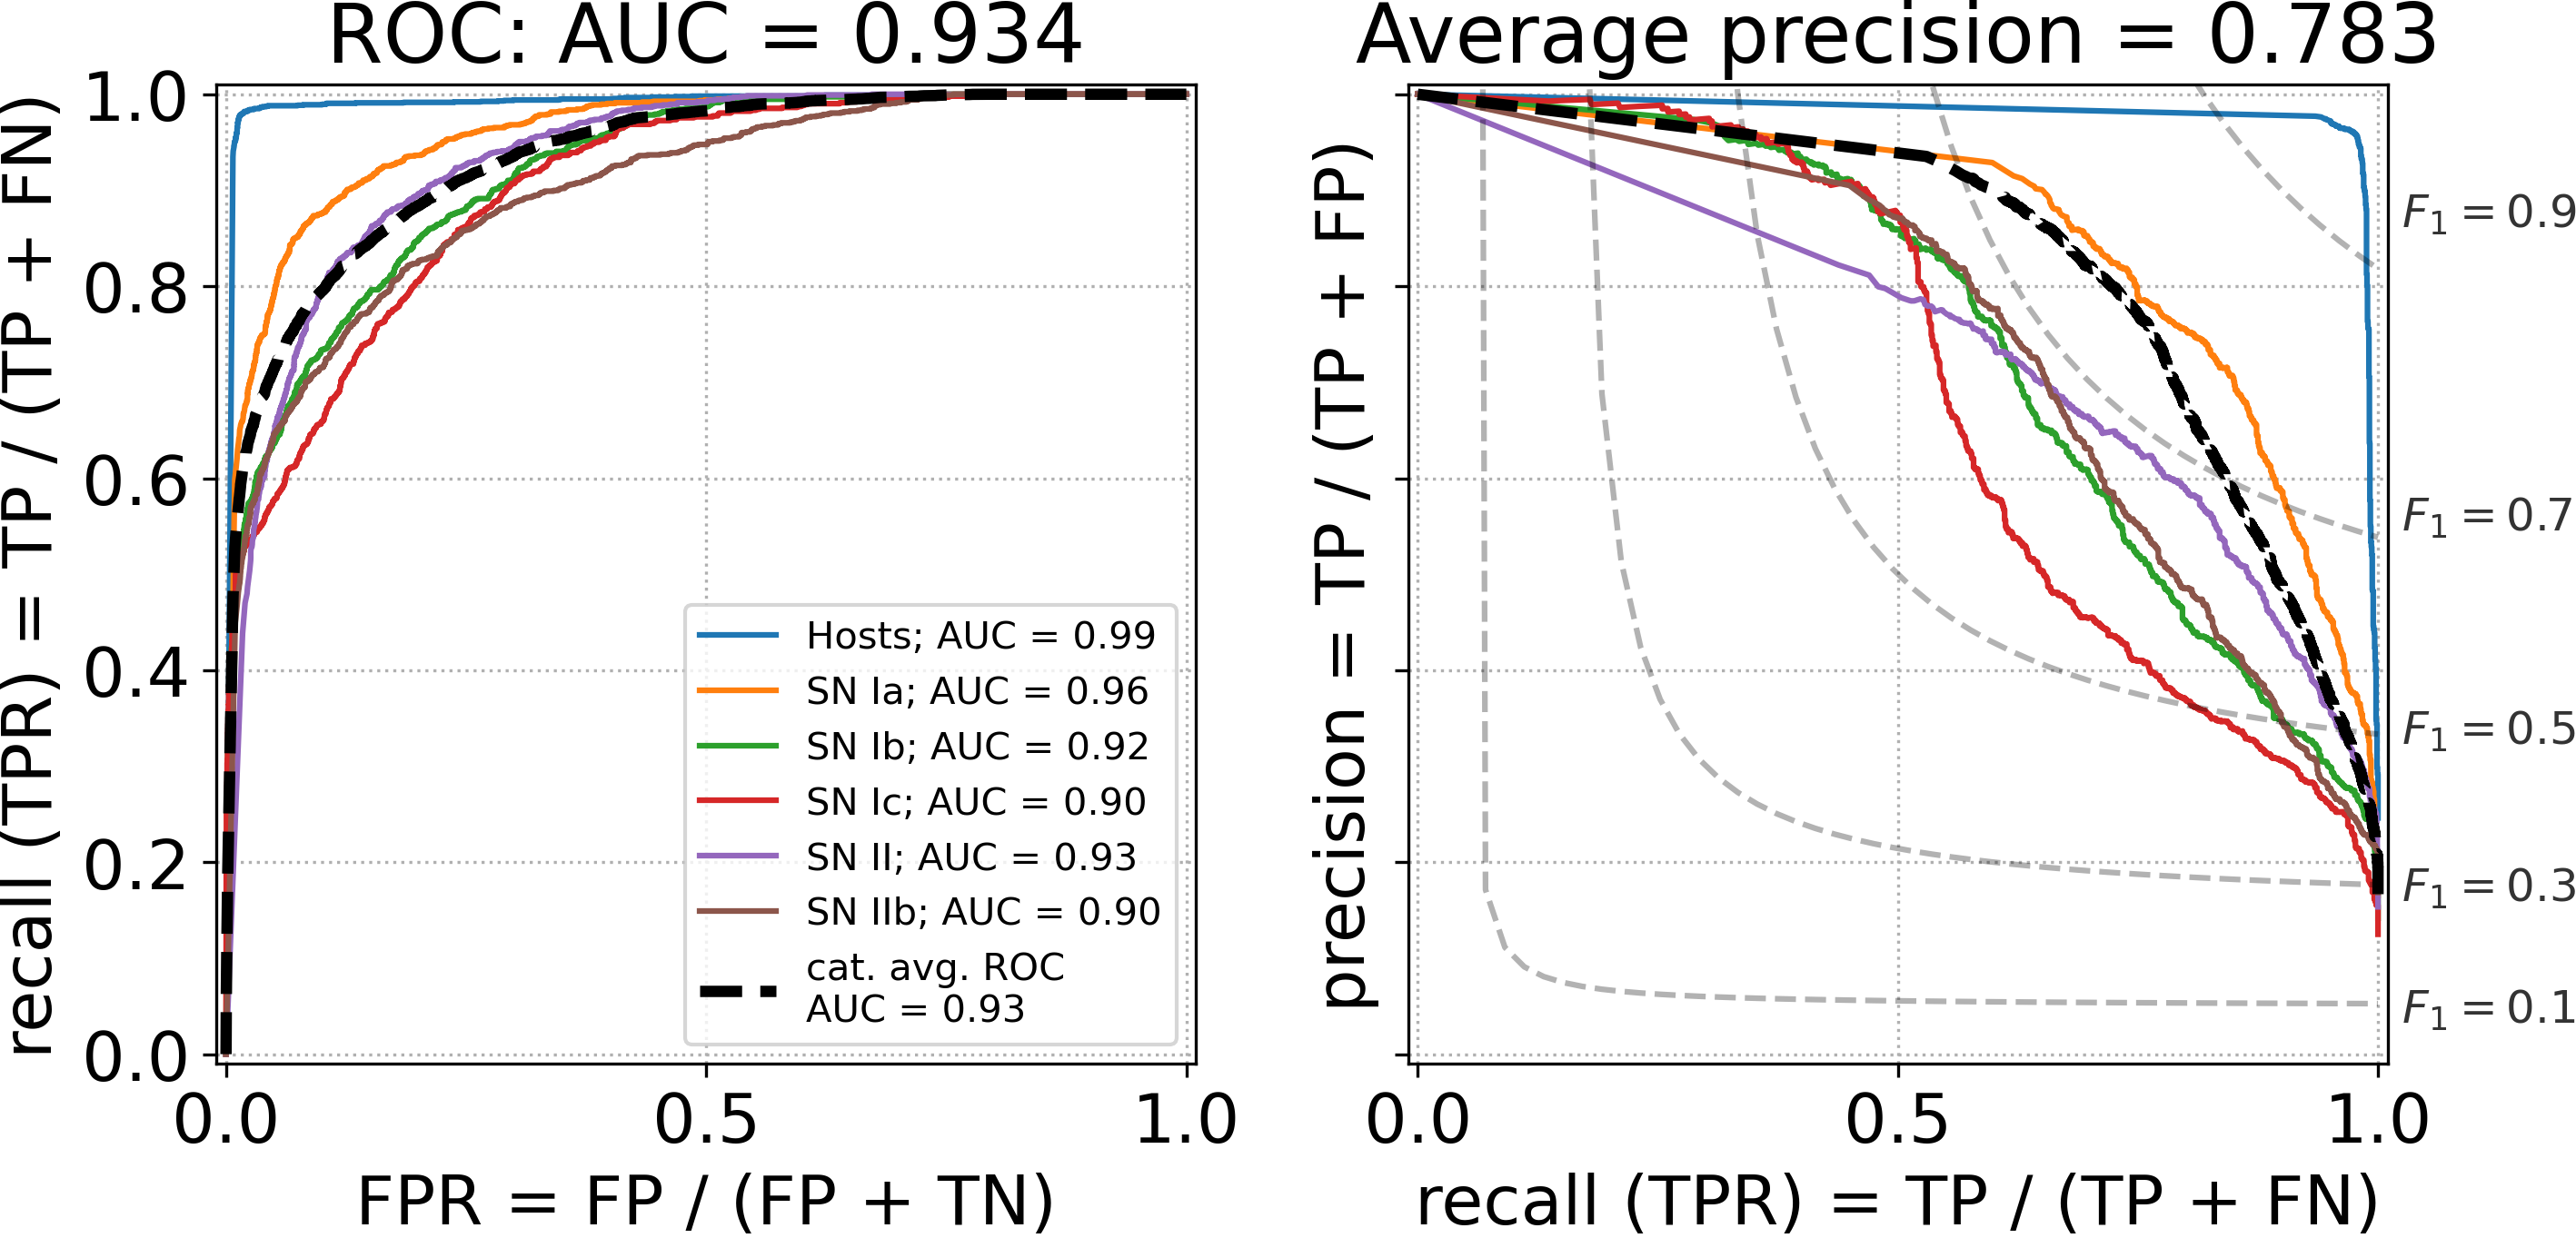
\includegraphics[height=4.3cm]{figures/v1_real/vit_model_V1_original_redoroc99_e31.png}
    \quad
    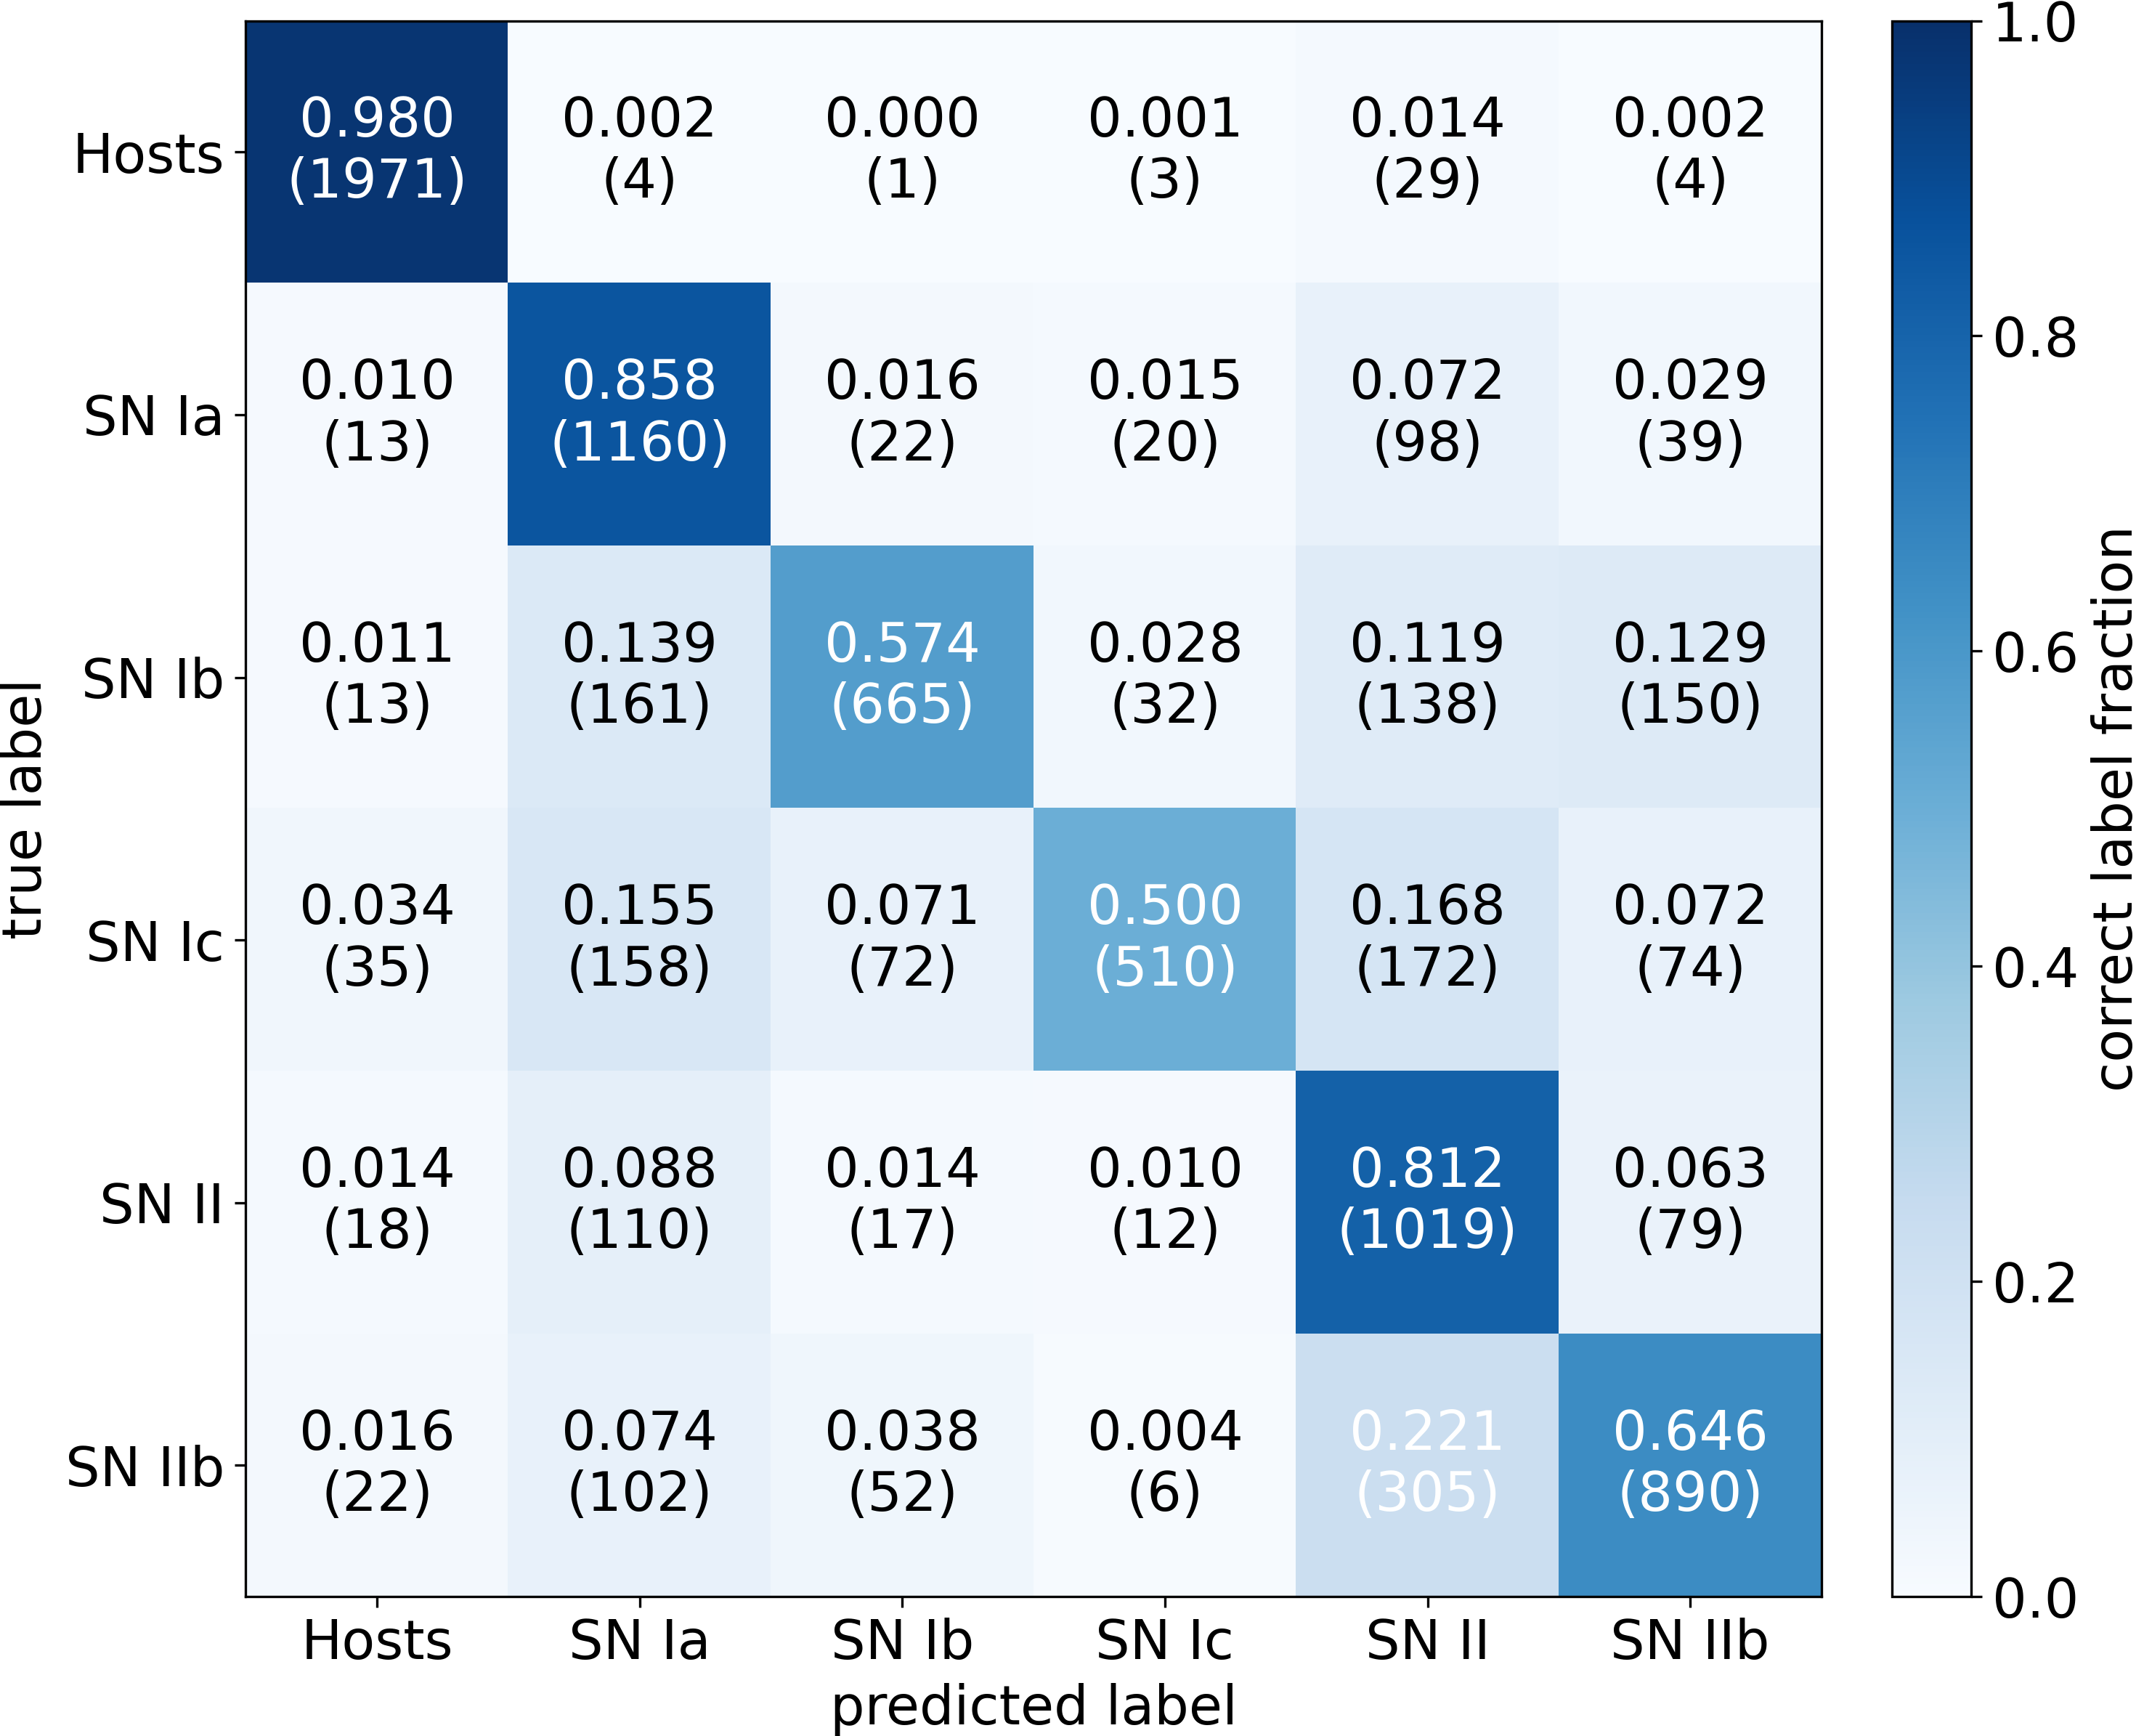
\includegraphics[height=4.3cm]{figures/v1_real/vit_model_V1_original_redocm99_e31.png}
    \caption{Spectral ViT V1 Diagnostics: ROC Curve (left) and Confusion Matrix (right) with a 99\% confidence
    cut \label{fig:v1_99_qual}}
\end{figure}

While the accuracy score didn't increase significantly with the second confidence cut, 
the important metric is the number of positive predictions made. All AUC scores 
are above 0.95, and the number of found targets is significantly higher than the 
CNN previously used. For example, Figure~\ref{fig:v1_999999_qual} correctly 
classifies 4705 targets, while Figure~\ref{fig:cnn_qual2} only correctly classifies 
3742 targets under a less strict confidence cut. This is a 26\% increase in the
number of correctly classified targets not excluded by the confidence cut.

\begin{figure}
    \centering
    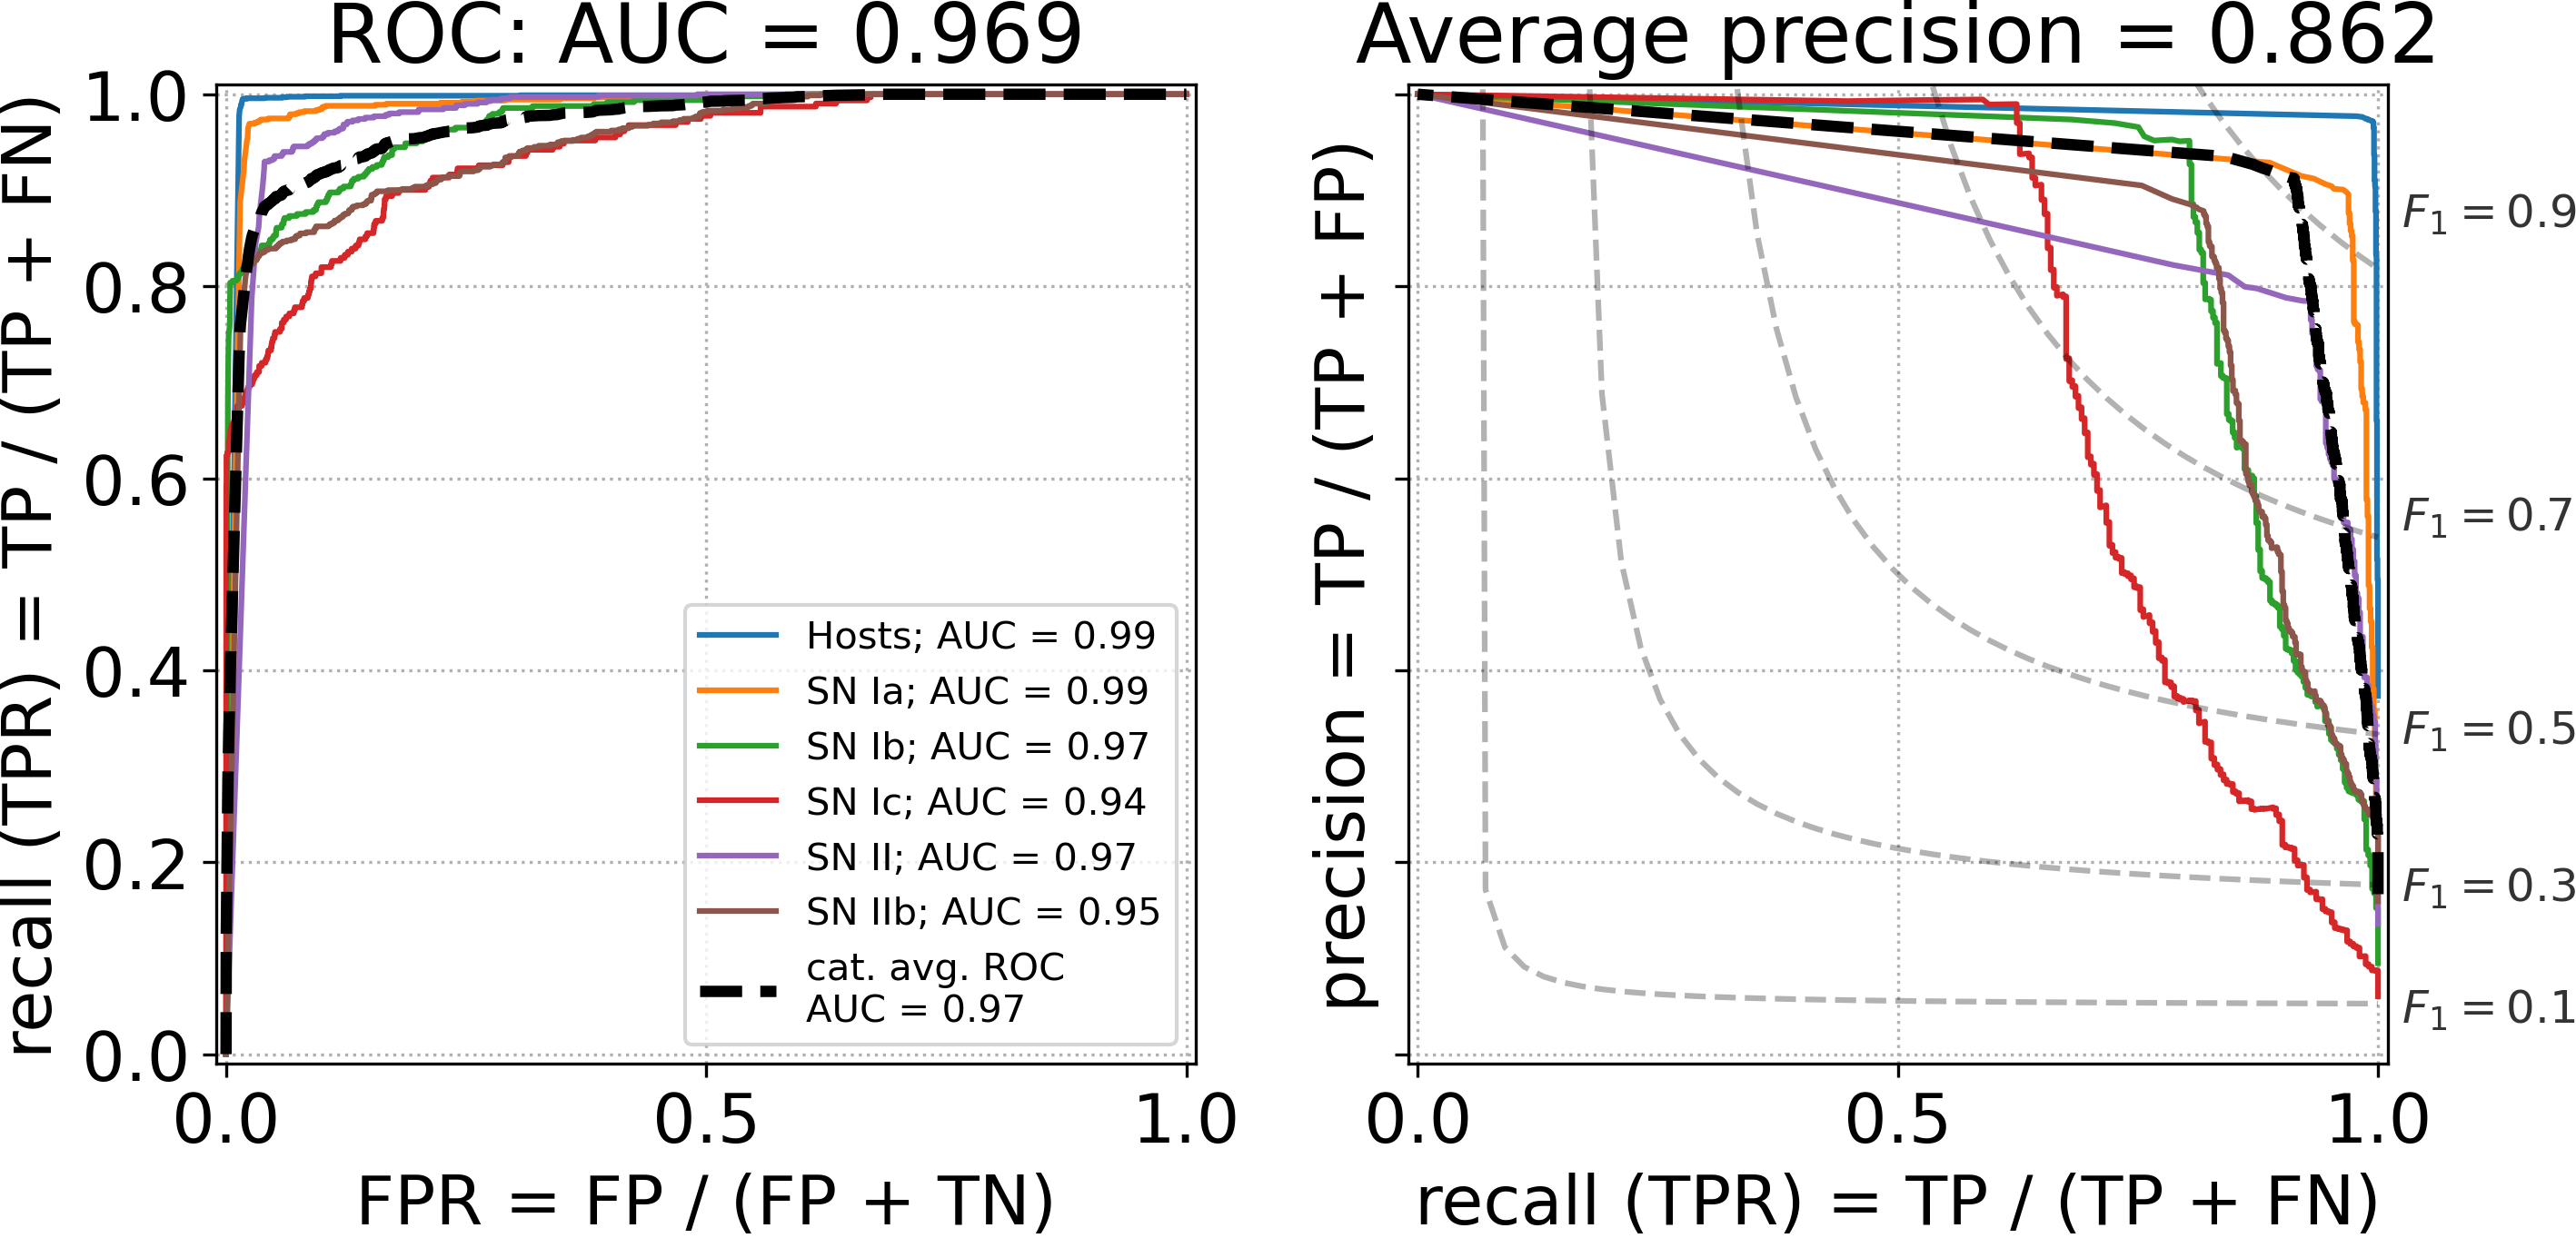
\includegraphics[height=4.3cm]{figures/v1_real/vit_model_V1_original_redoroc999999_e31.png}
    \quad
    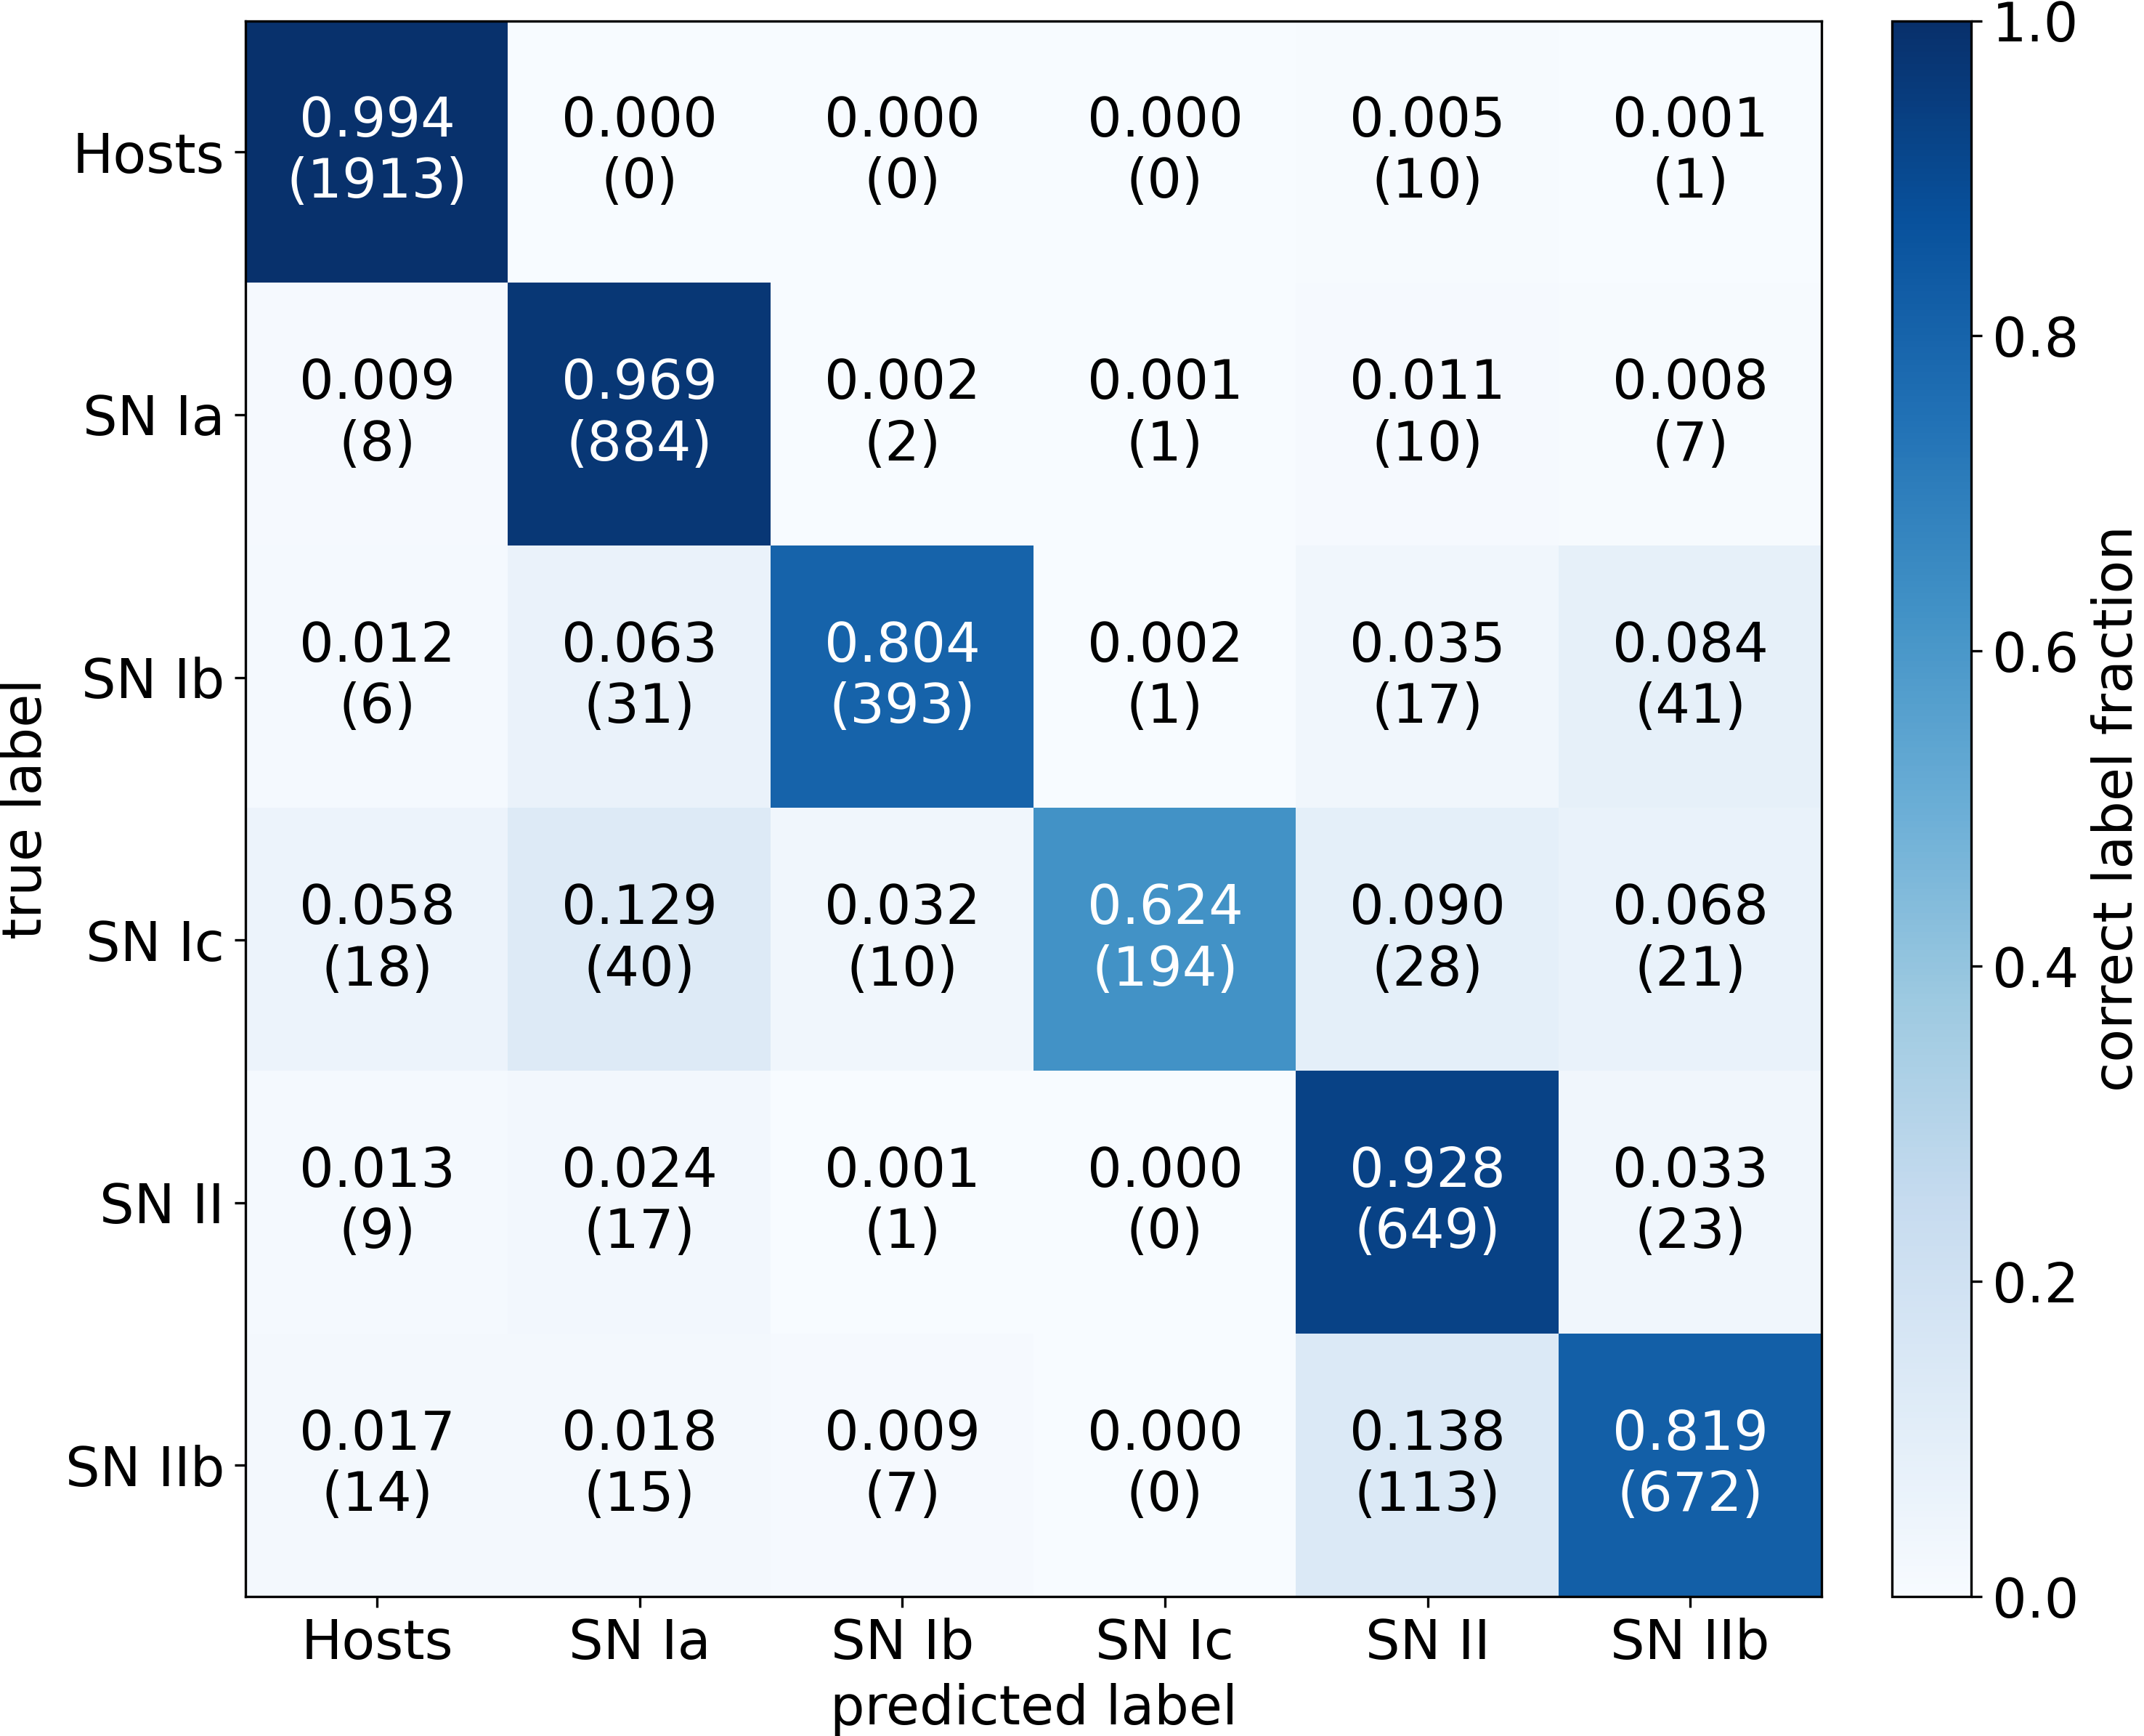
\includegraphics[height=4.3cm]{figures/v1_real/vit_model_V1_original_redocm999999_e31.png}
    \caption{Spectral ViT V1 Diagnostics: ROC Curve (left) and Confusion Matrix (right) with a 99.9999\% confidence
    cut \label{fig:v1_999999_qual}}
\end{figure}

% \clearpage
\section{V2}
\begin{figure}[b]
    \centering
    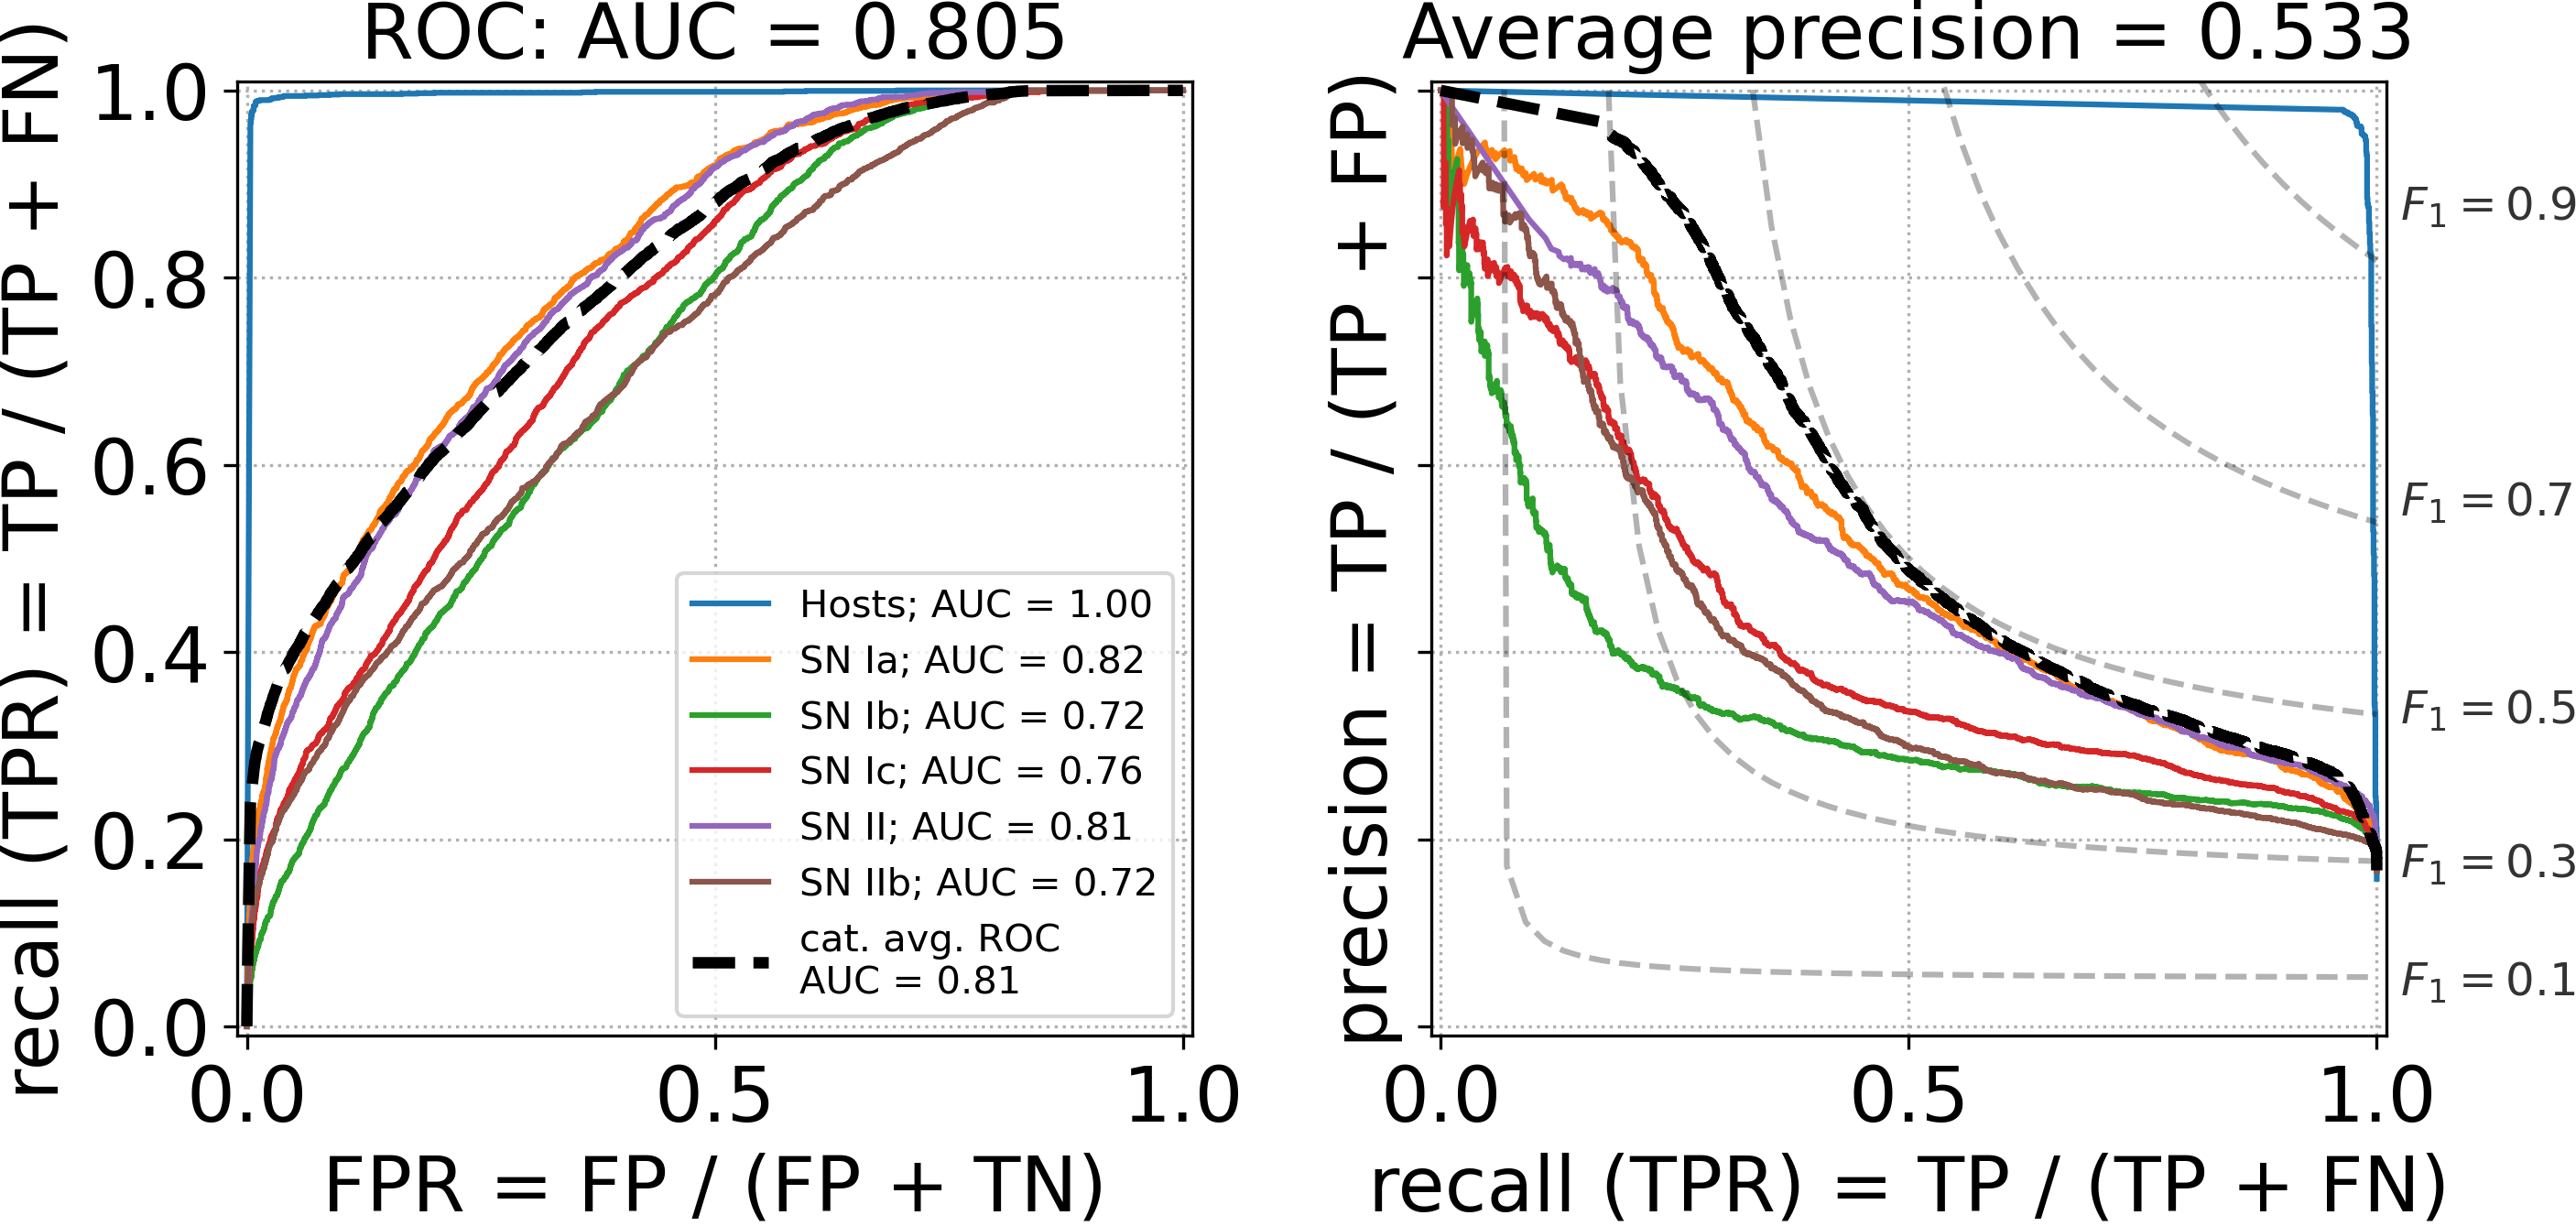
\includegraphics[height=4.3cm]{figures/v2_real/vit_model_V2rocfulle_e26.png}
    \quad
    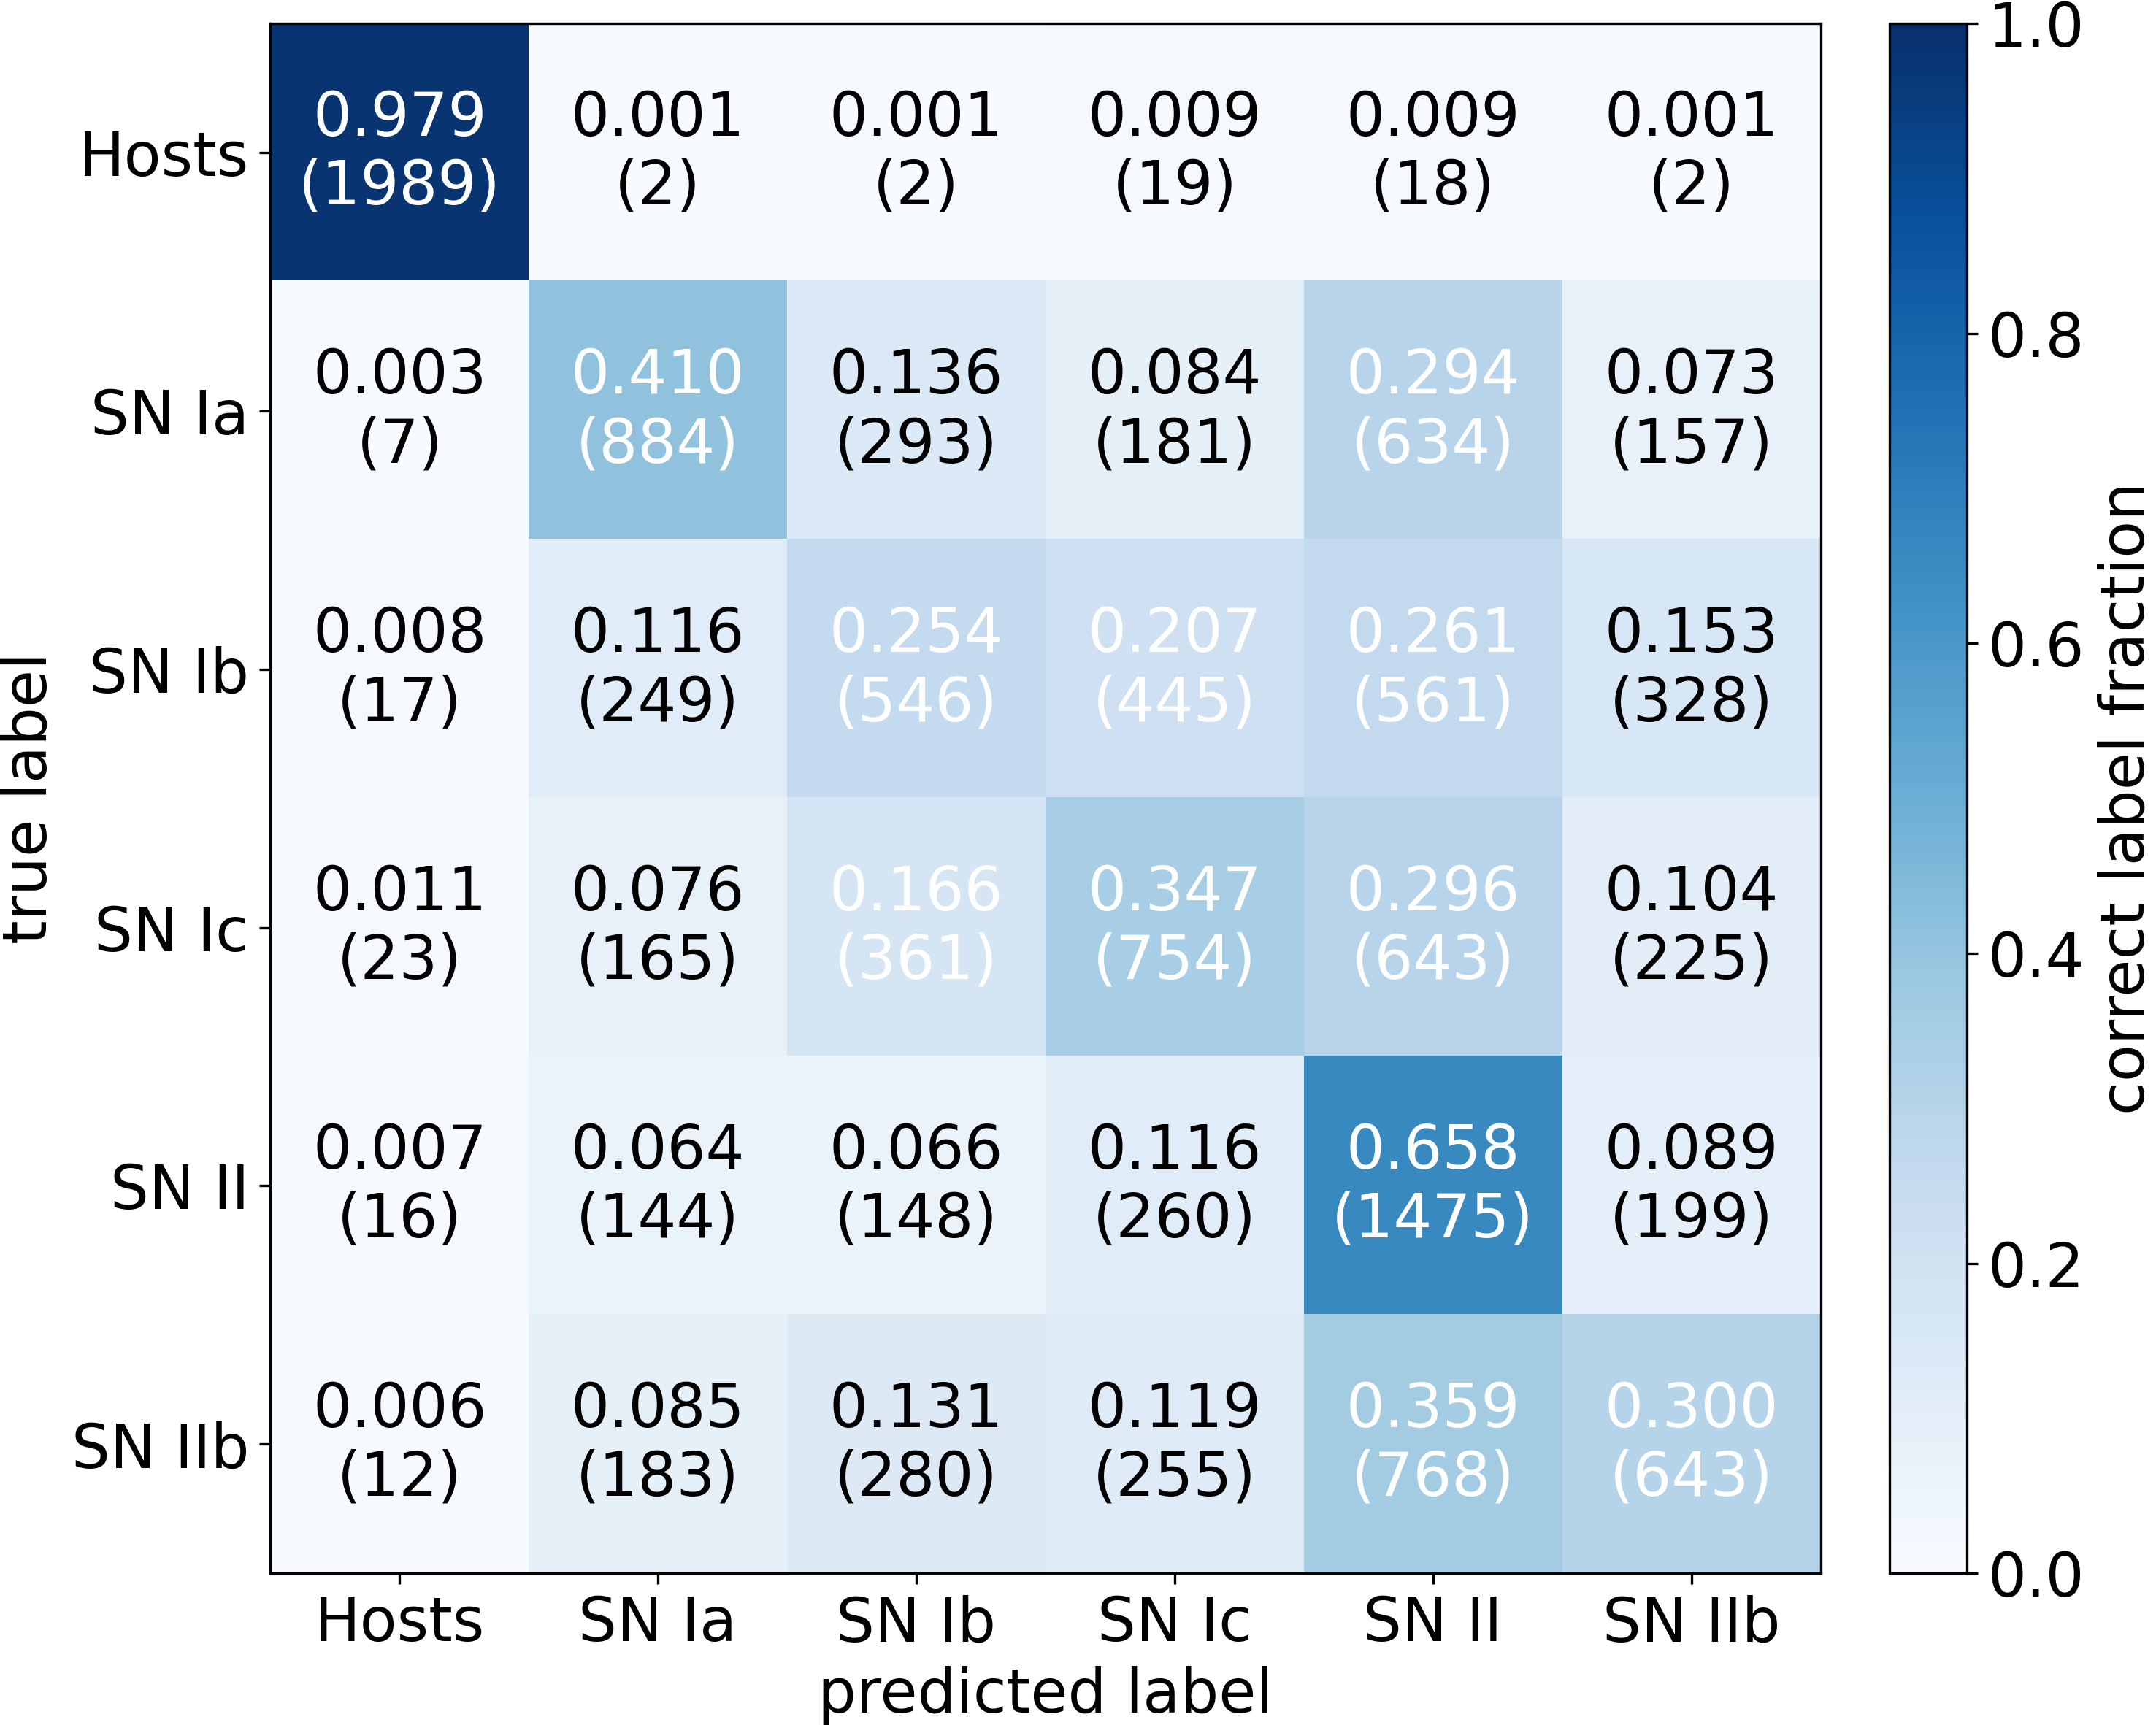
\includegraphics[height=4.3cm]{figures/v2_real/vit_model_V2cmfull_e26.png}
    \caption{Spectral ViT V2 Diagnostics: ROC Curve (left) and Confusion Matrix (right)\label{fig:v2_qual}}
\end{figure}
The goal of the Spectral ViT V2 was to see if the dependence on the redshift fit 
provided by the DESI pipeline could be removed. The validation set was the same size 
as the V1 validation set, 12888 specra. The ROC curve and confusion matrix are shown
in Figure~\ref{fig:v2_qual}. Classification of SNe and non-SNe is still very good,
with an AUC of 1.0, but the other classes are not classified as well, resulting in 
an overall AUC of 0.805 and a lower average precision of 0.533. 


Similar to the CNN, on a 99\% confidence cut, only 34\% of the original predictions
remain (Figure~\ref{fig:v2_max}). The AUC score and average precision both increase, as shown in Figure~\ref{fig:v2_99_qual}, 
but the important metric is the number of positive predictions made. The ViT, 
despite not looking at spectra in the rest frame, was still able to identify more 
Host and SN II spectra than the CNN, but not as many of the other spectra. 


\begin{figure}[t]
    \centering
    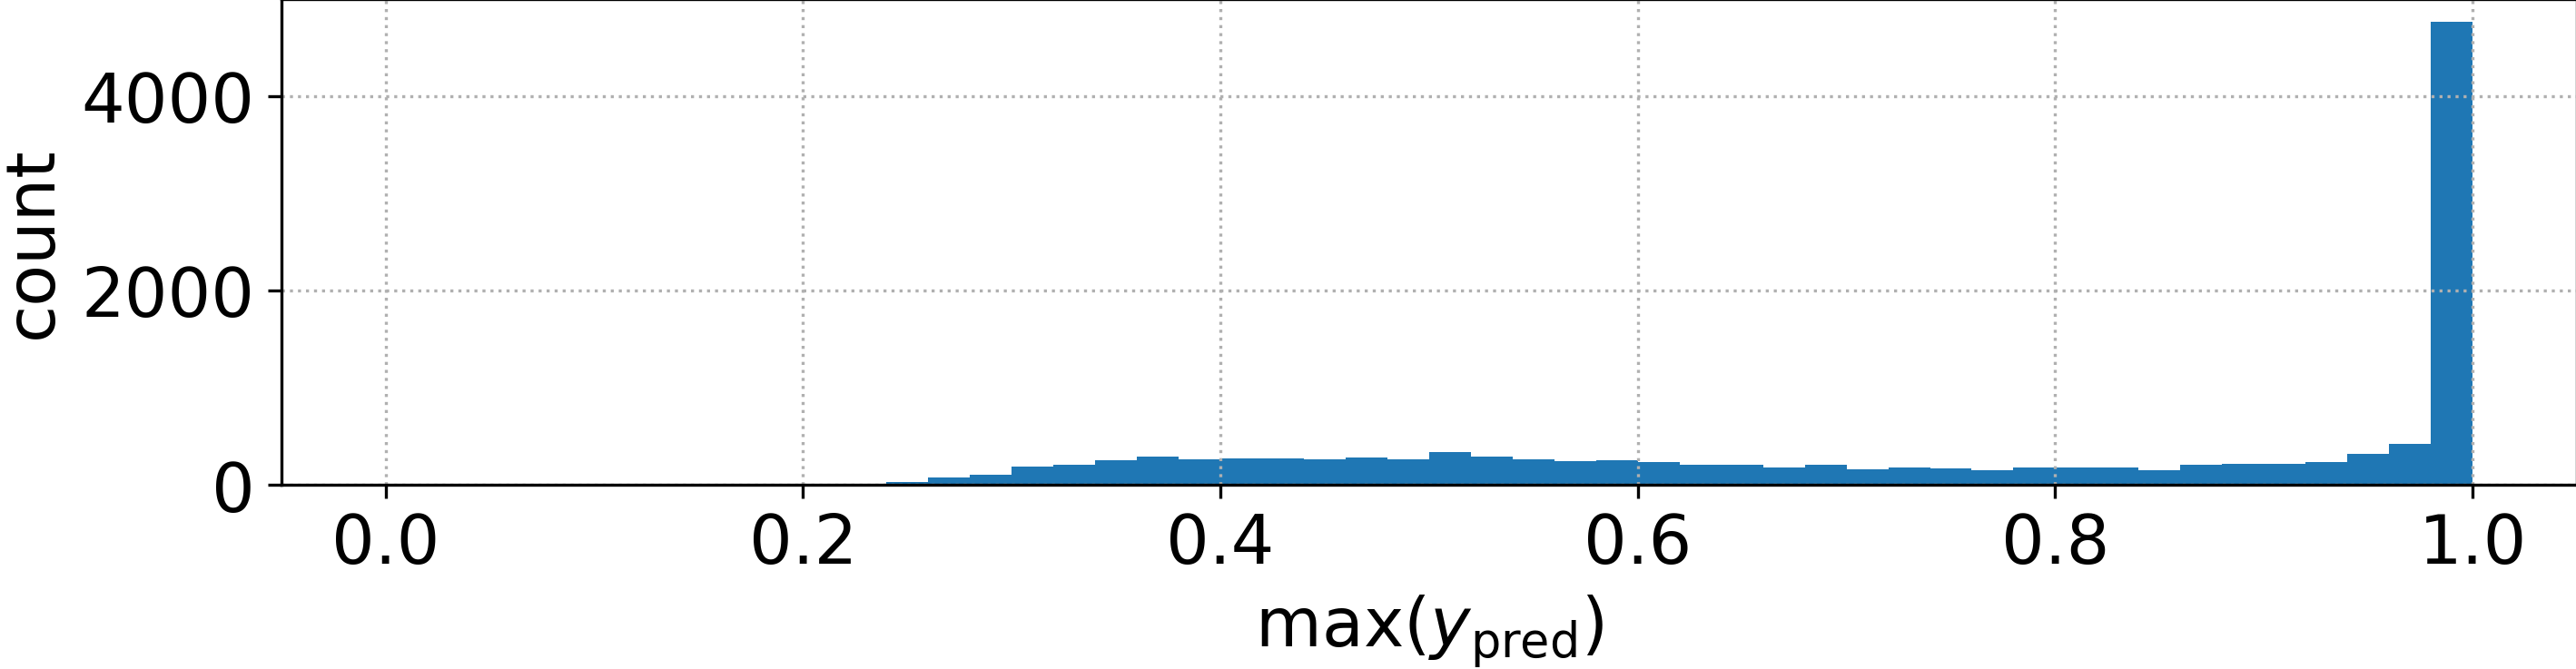
\includegraphics[width=0.6\textwidth]{figures/v2_real/vit_model_V2max_ypred_26.png}
    \caption{Max value of the output vector from the Spectral ViT V2.\label{fig:v2_max}}
\end{figure}

This, combined with the lower AUC score, indicates that the ViT V2 is not a suitable 
replacement for the ViT V1 for the purposes of this project. However, the ViT V2
is still able to identify SNe and non-SNe spectra with high accuracy, and could
be used as a classifier for these two classes. 

\begin{figure}[h]
    \centering
    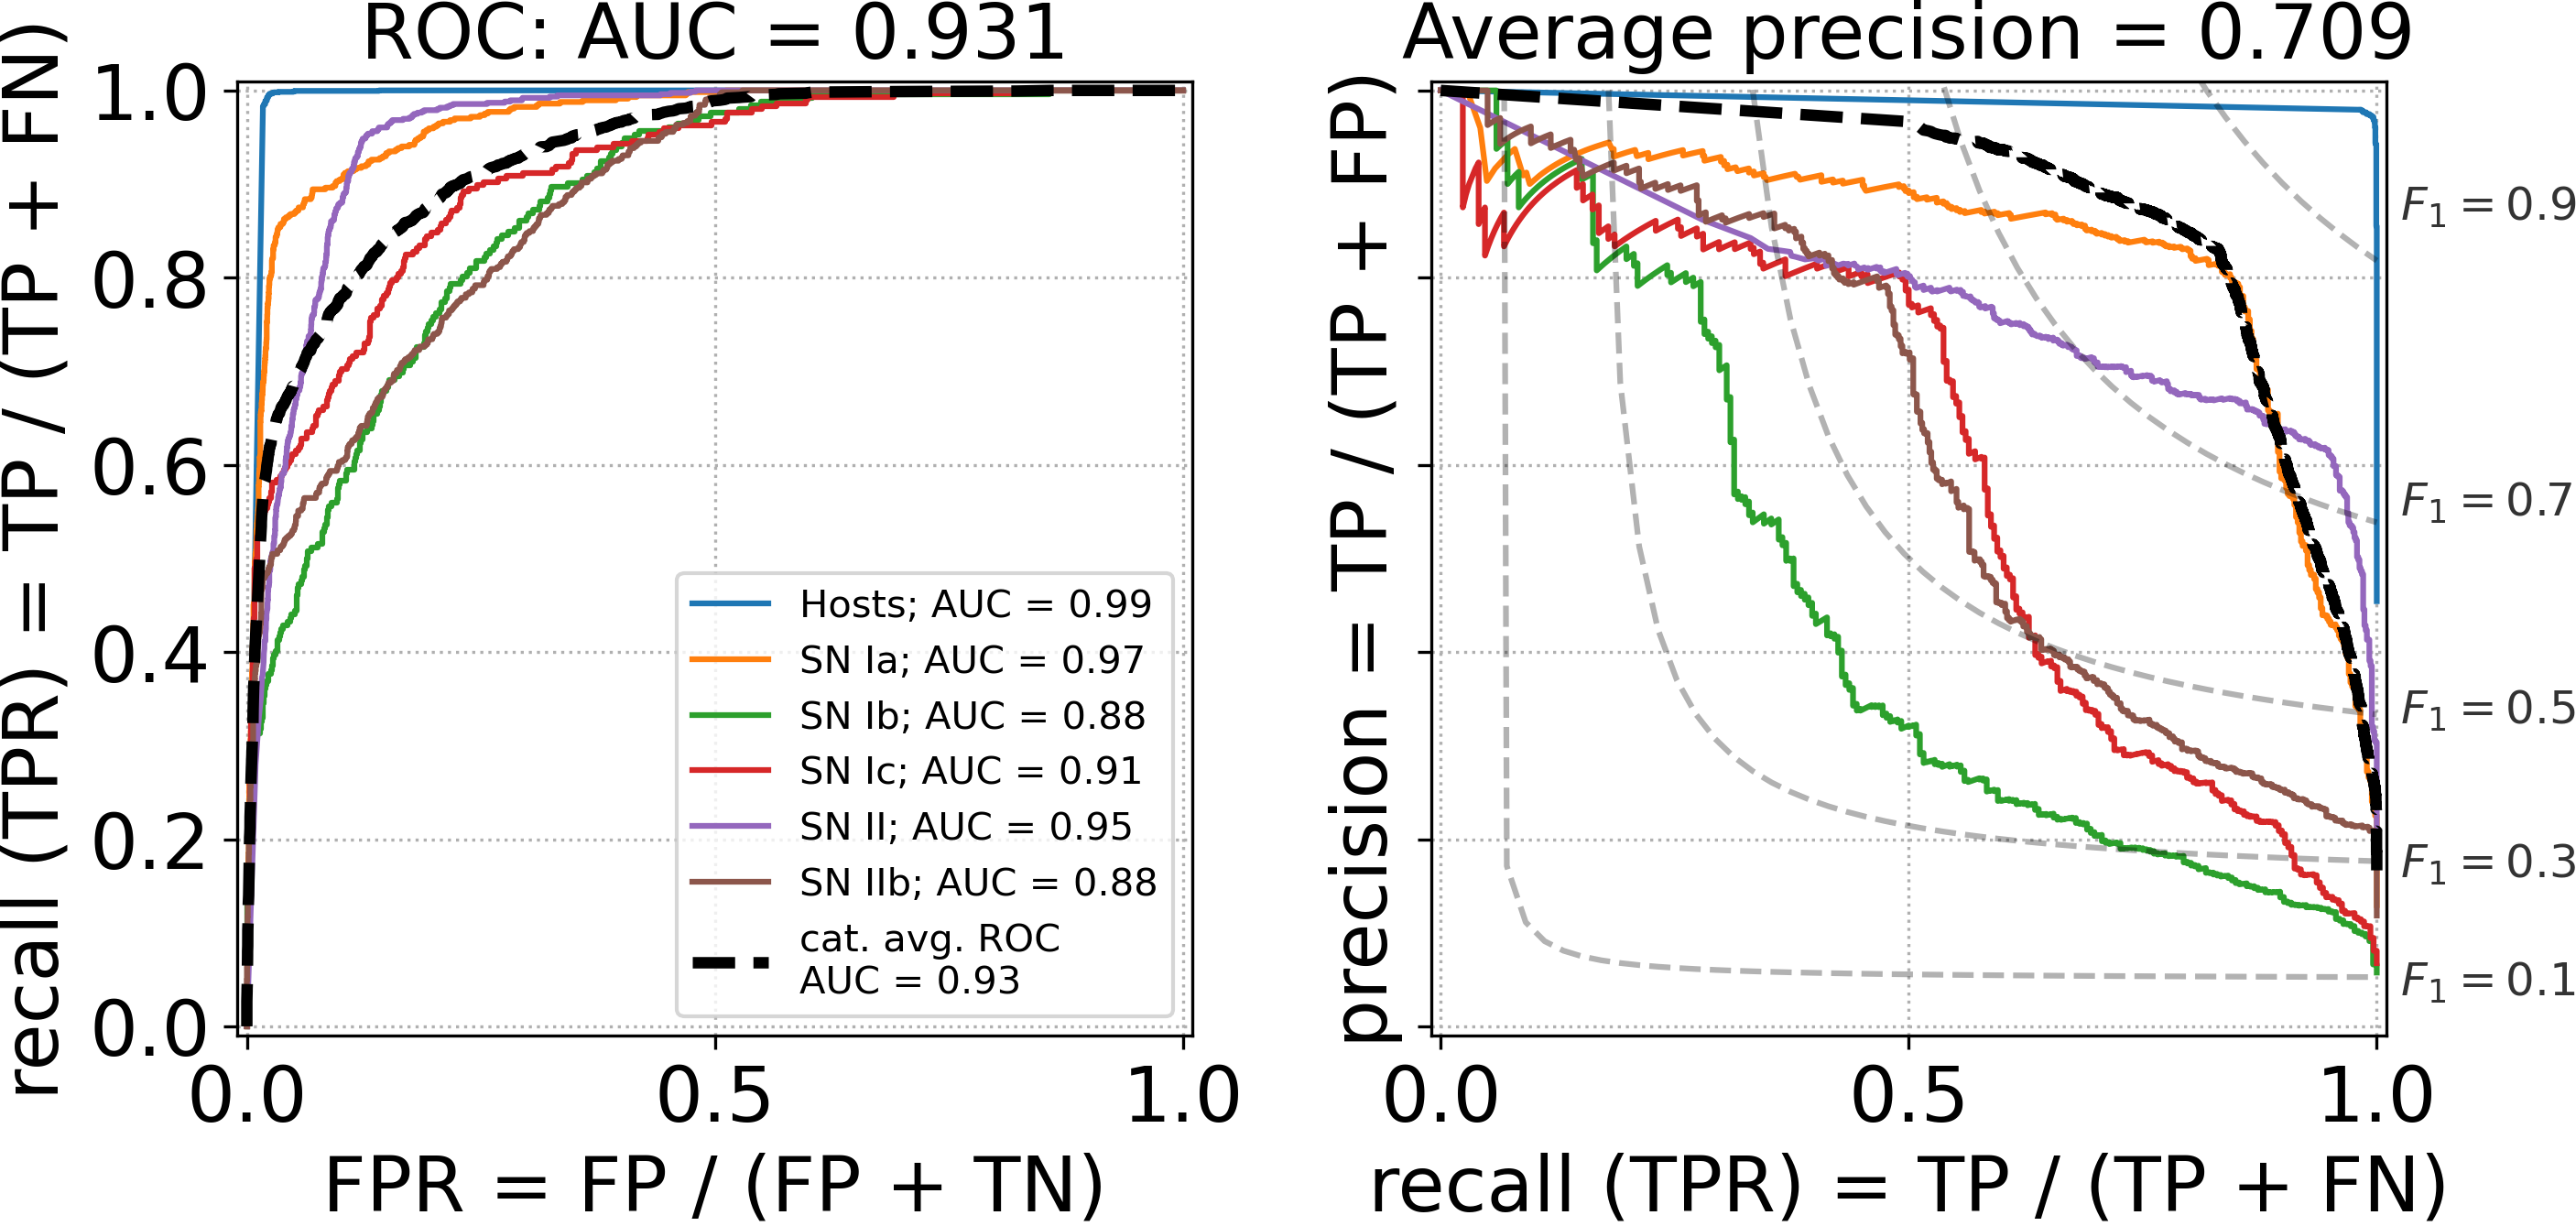
\includegraphics[height=4.3cm]{figures/v2_real/vit_model_V2roc99_e26.png}
    \quad
    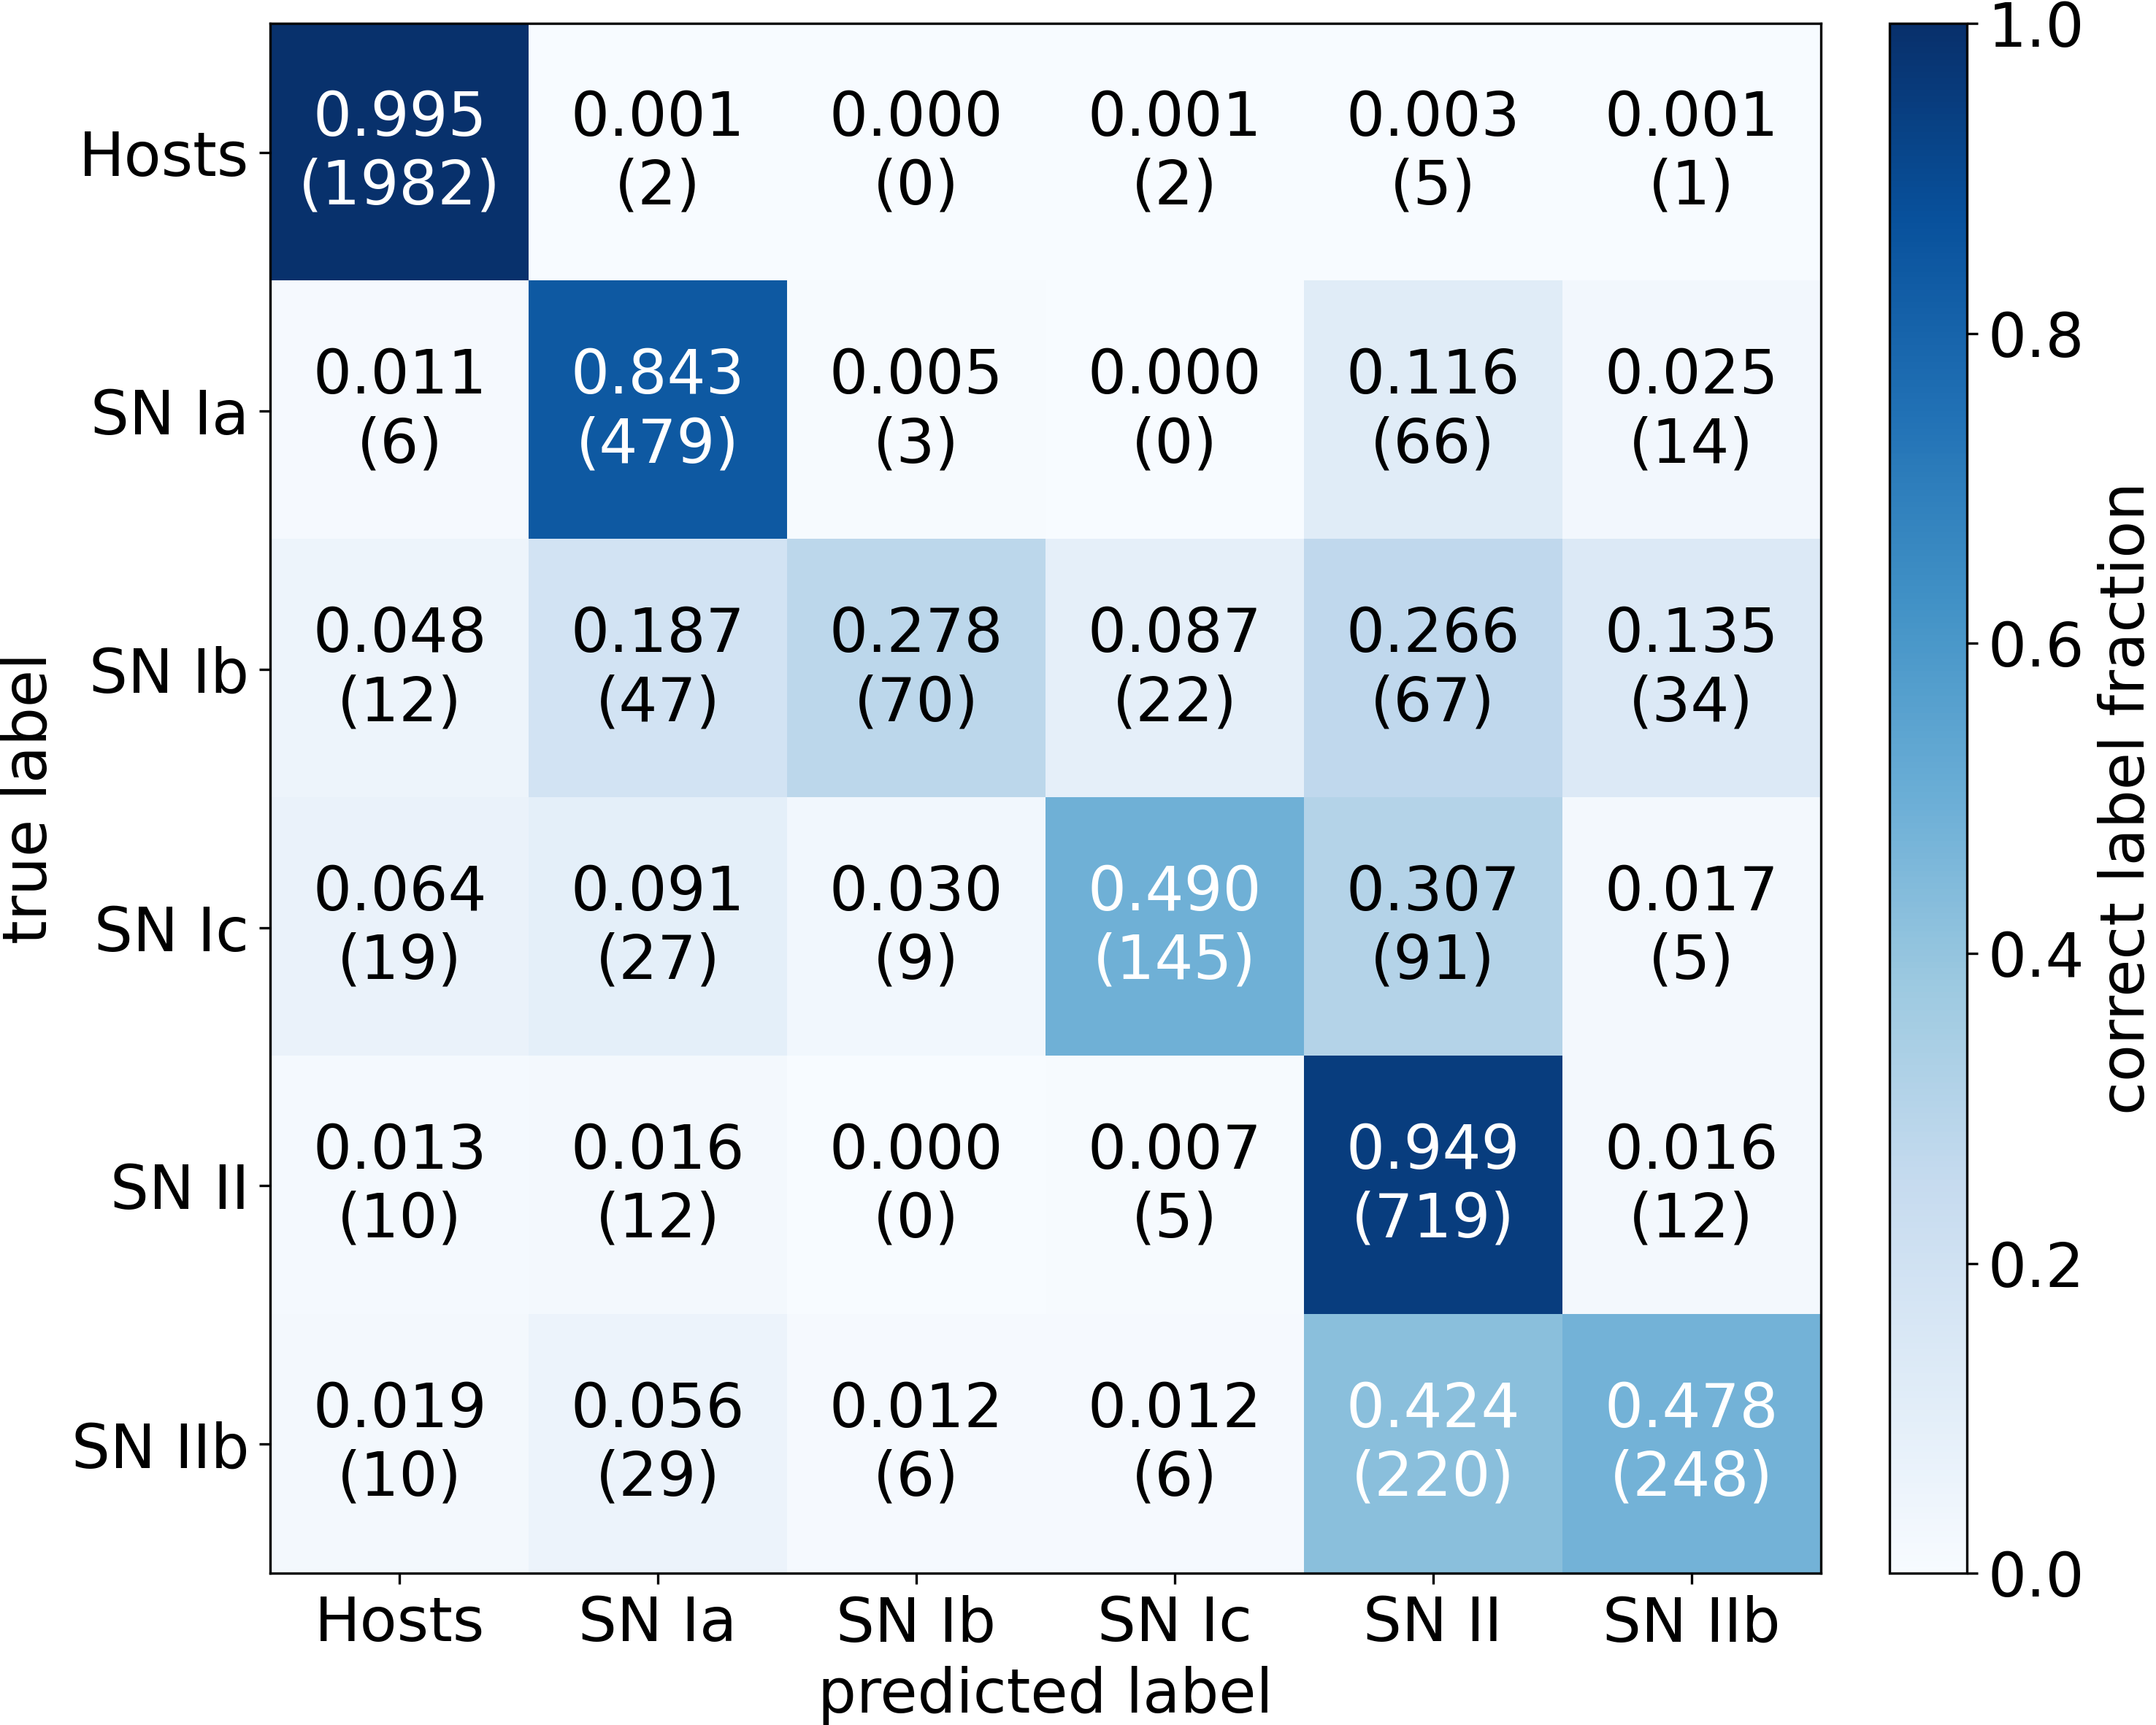
\includegraphics[height=4.3cm]{figures/v2_real/vit_model_V2cm99_e26.png}
    \caption{Spectral ViT V2 Diagnostics: ROC Curve (left) and Confusion Matrix (right) with a 99\% confidence
    cut\label{fig:v2_99_qual}}
\end{figure}



\clearpage
\subsection{Binary Classification}
To test the binary classification, the probabilities of all classes apart from 
non-SNe were summed. This resulted in a very high AUC score of 0.997, with a 
nearly perfect average precision of 0.987 (Figure \ref{fig:v2_binary_qual}).
This, combined with the high number of confident predictions shown in 
Figure~\ref{fig:v2_max}, indicates the ViT V2's ability to act as a binary 
classifier for SNe.
\begin{figure}[t]
    \centering
    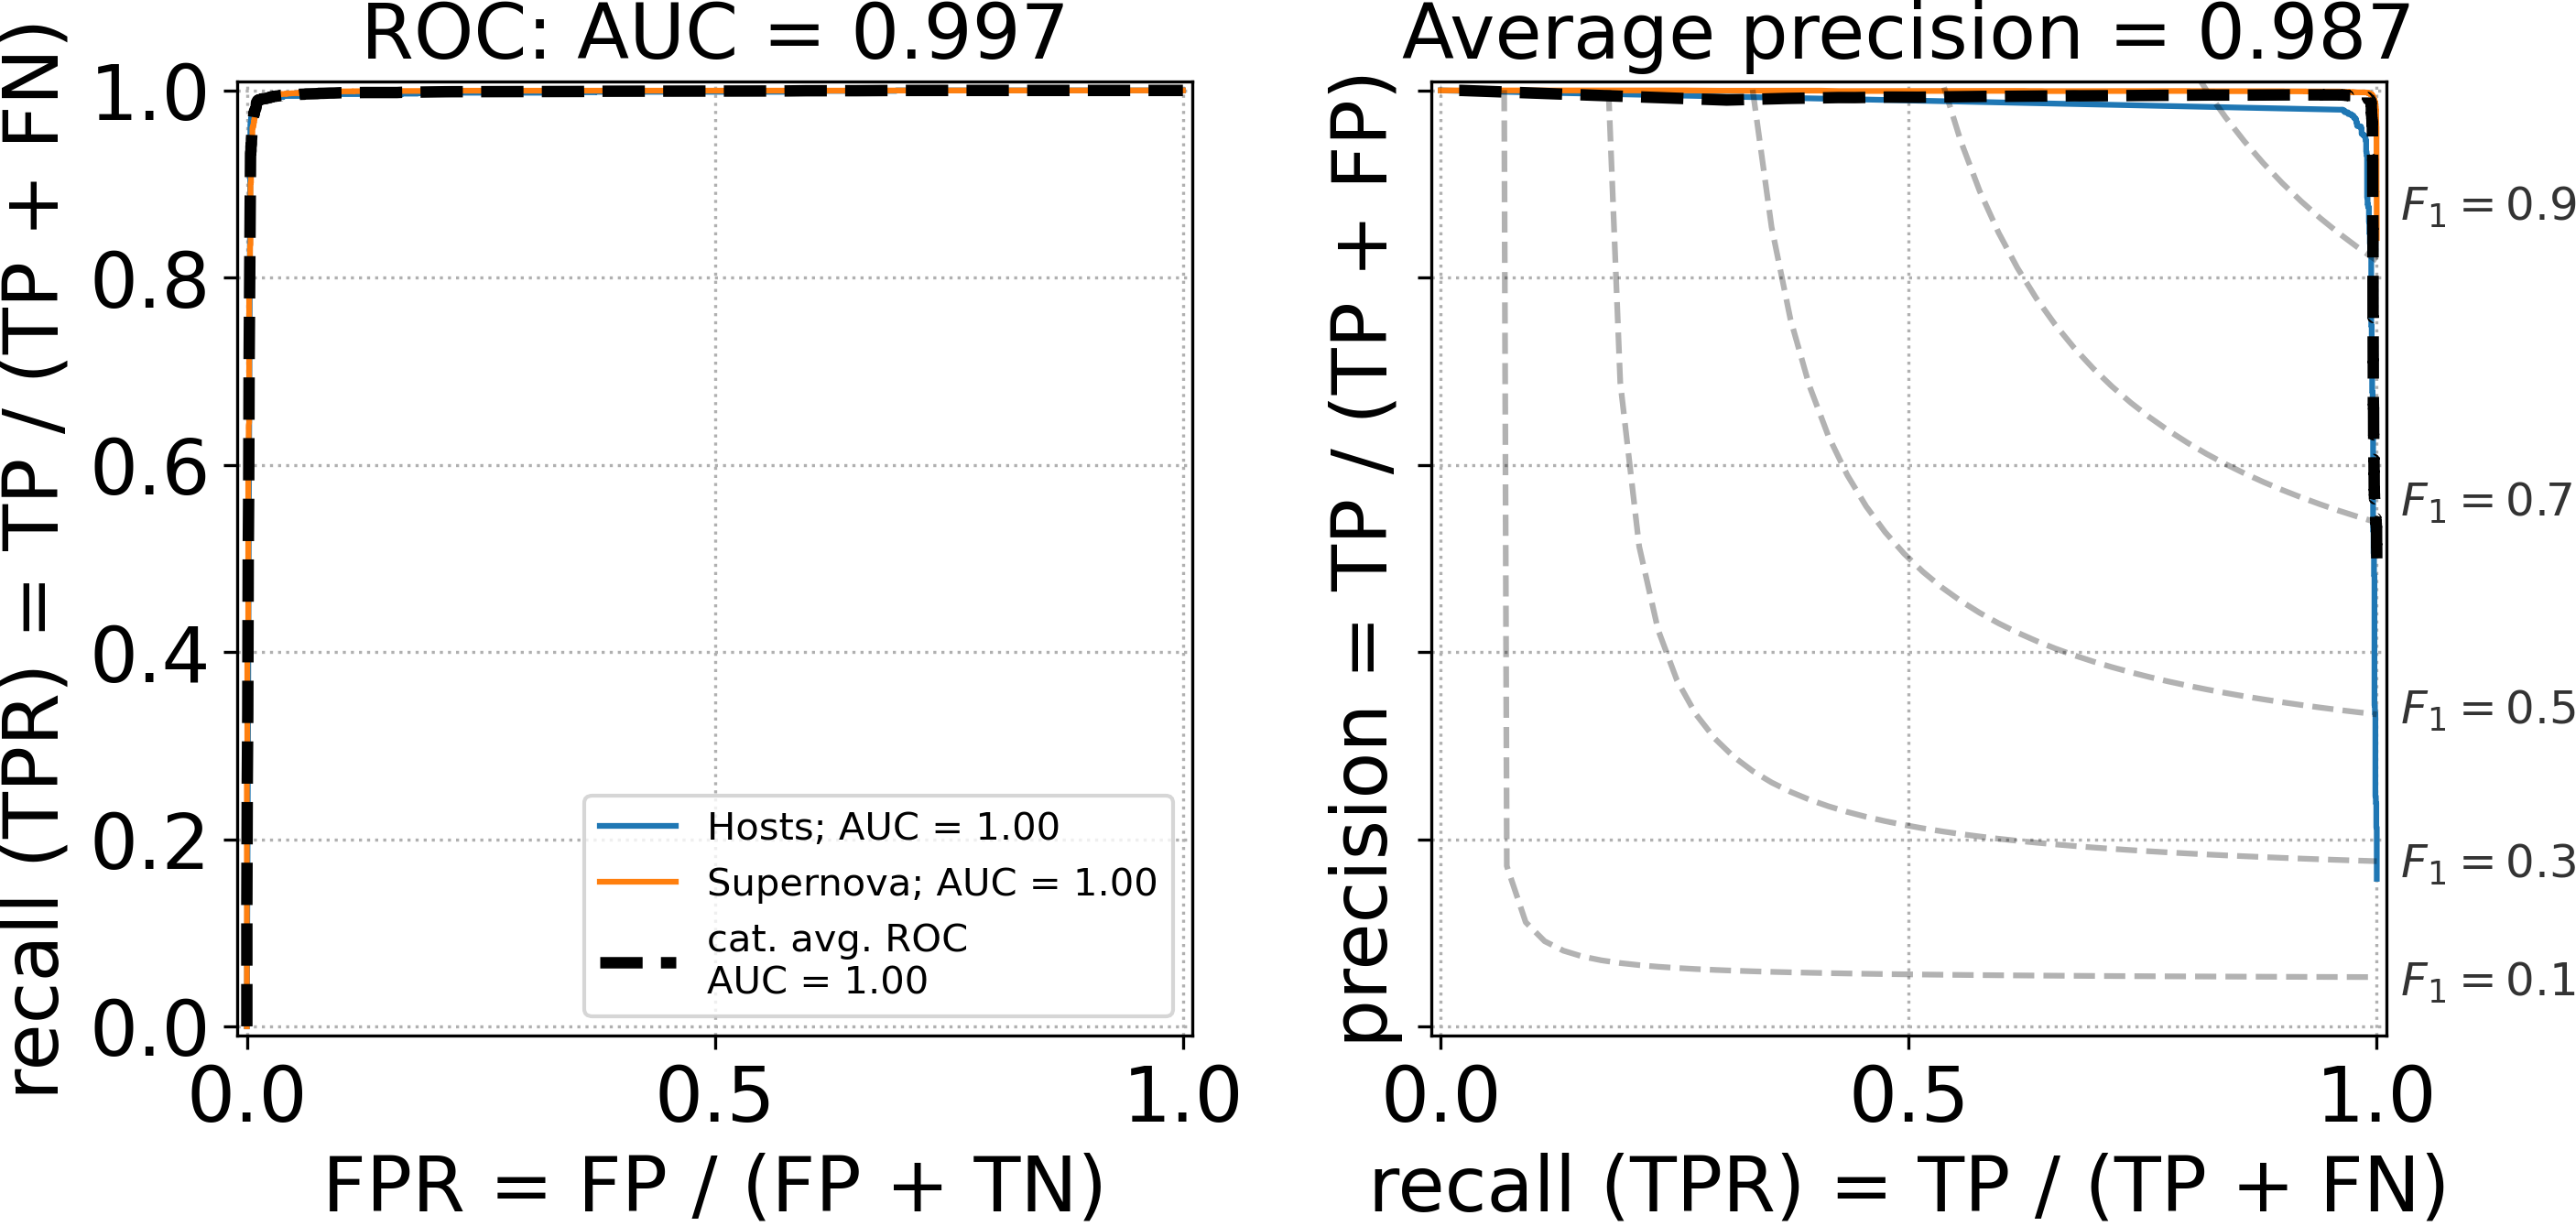
\includegraphics[height=4.2cm]{figures/v2_real/vit_model_V2rocfull_binary_e26.png}
    \quad
    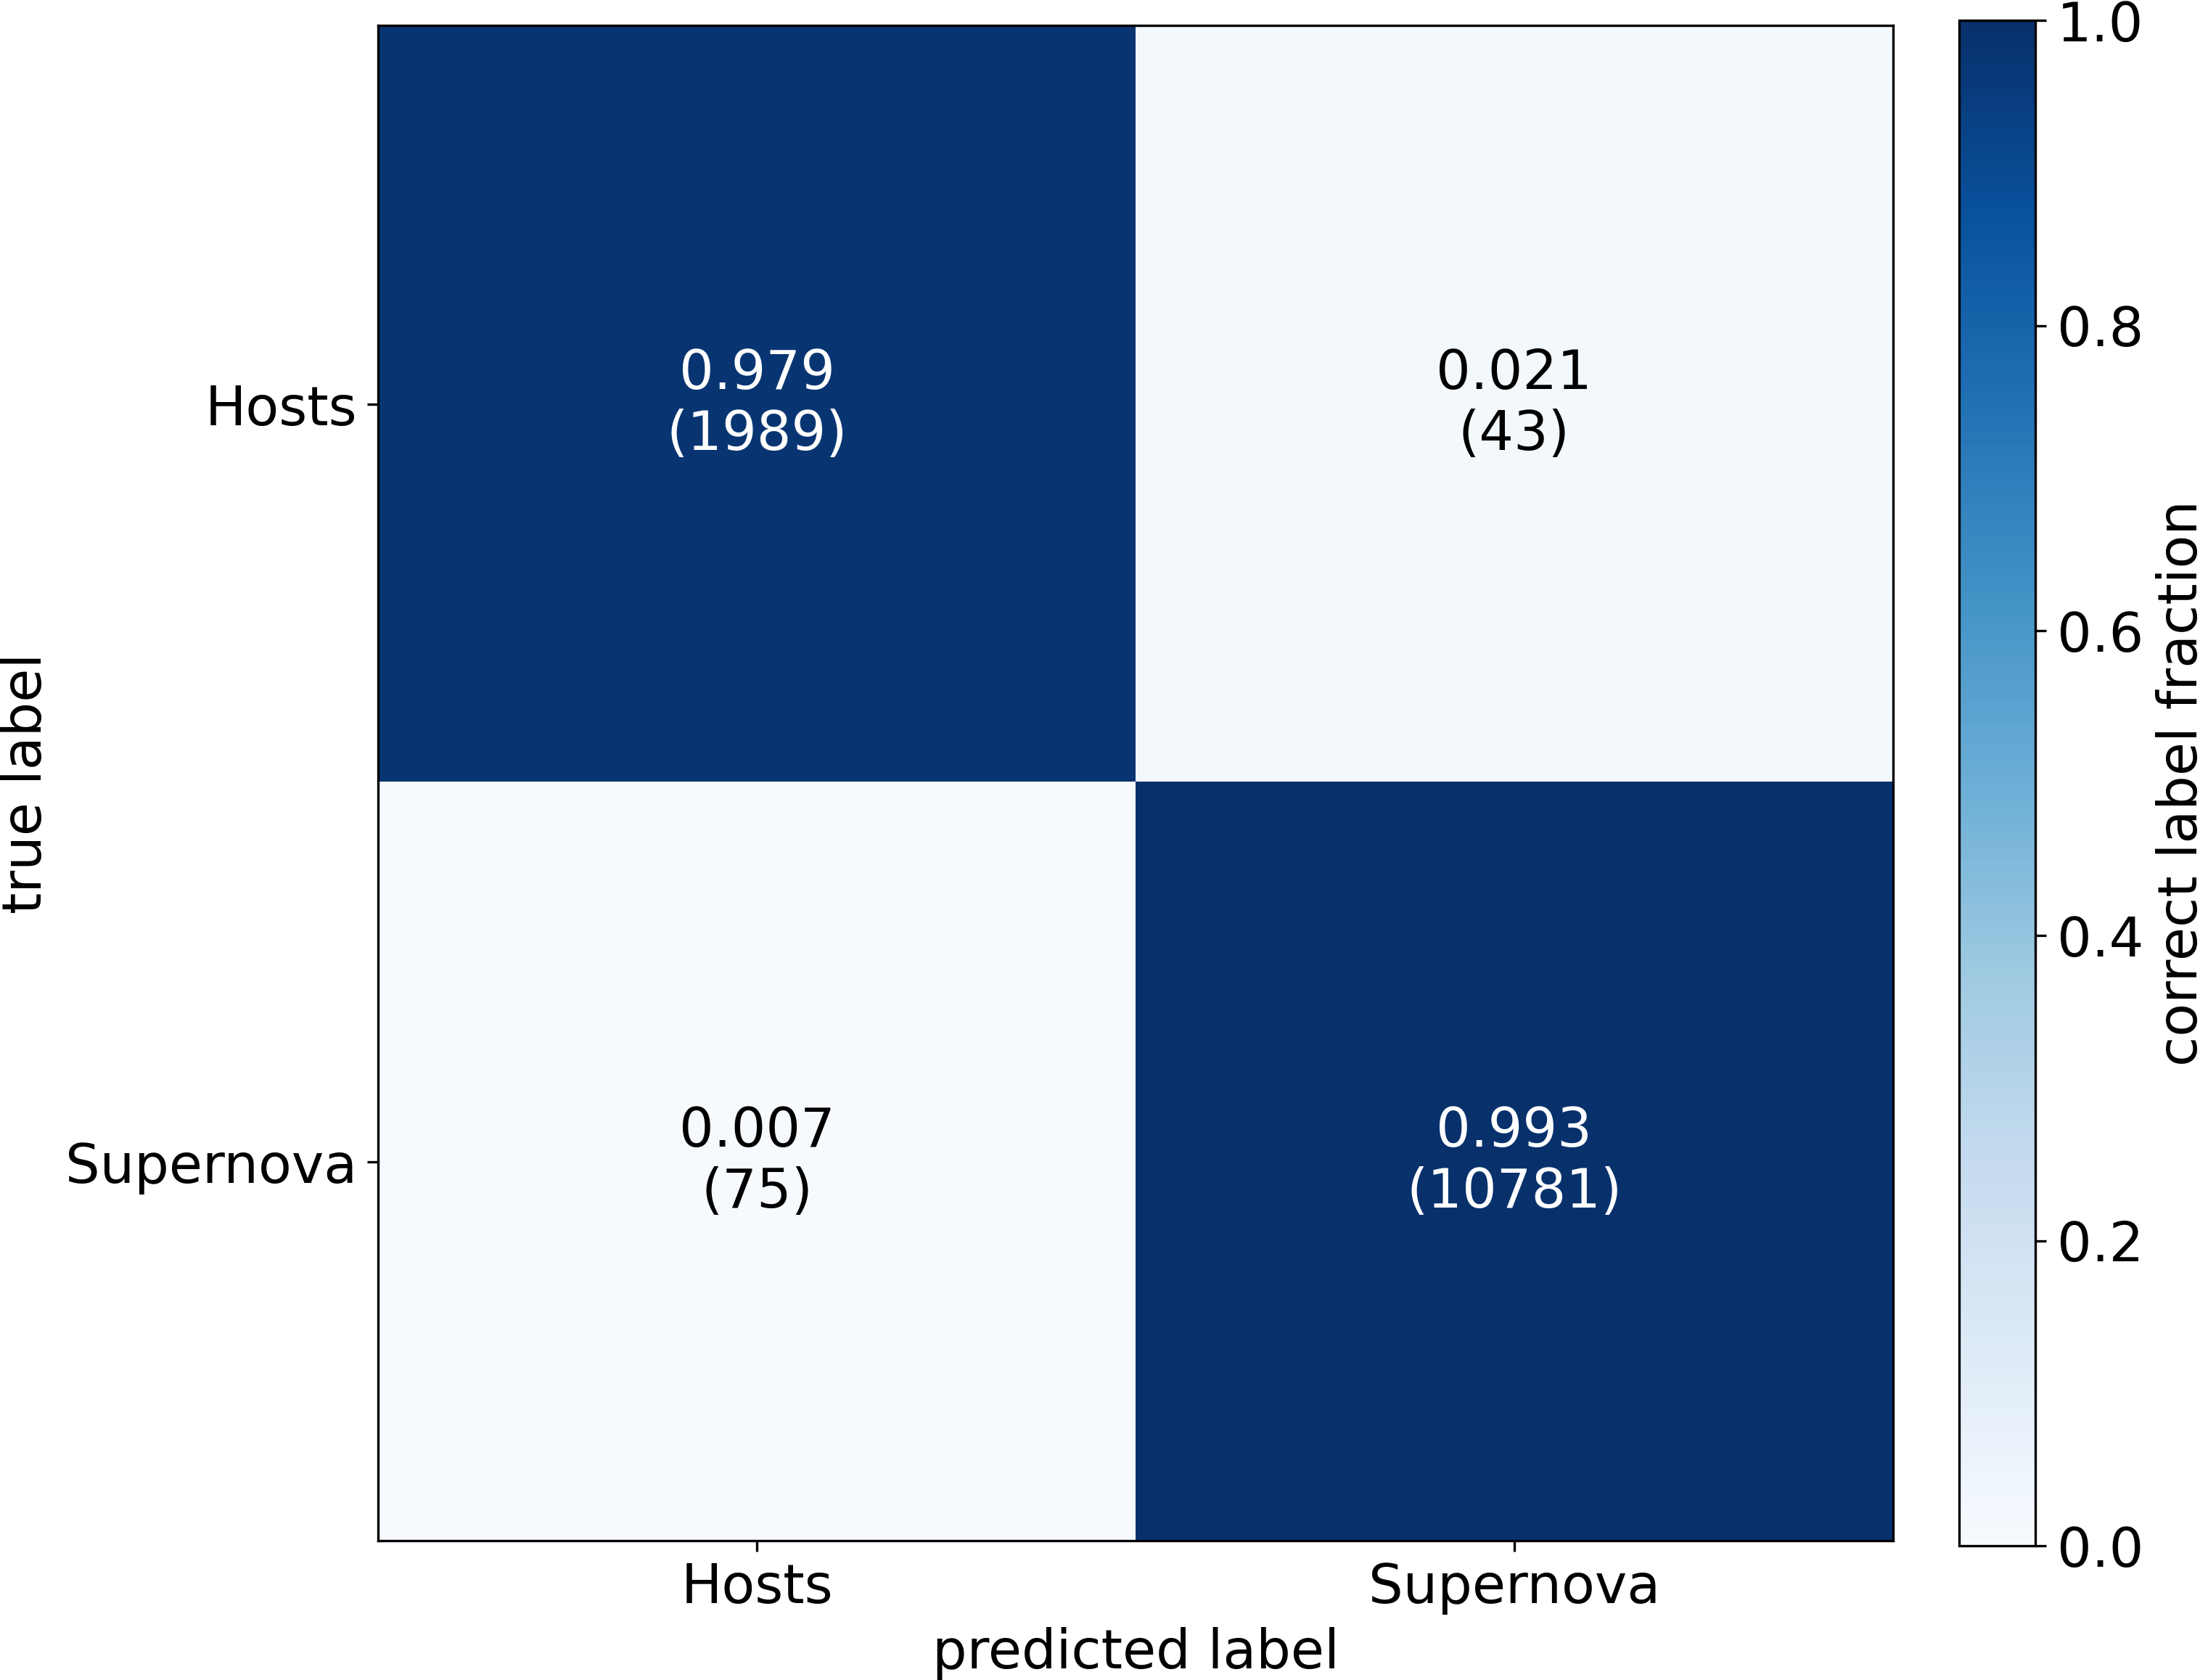
\includegraphics[height=4.2cm]{figures/v2_real/vit_model_V2cmfull_binary_e26.png}
    \caption{Spectral ViT V2 Binary Diagnostics: ROC Curve (left) and Confusion Matrix (right)\label{fig:v2_binary_qual}}
\end{figure}

\begin{figure}[h]
    \centering
    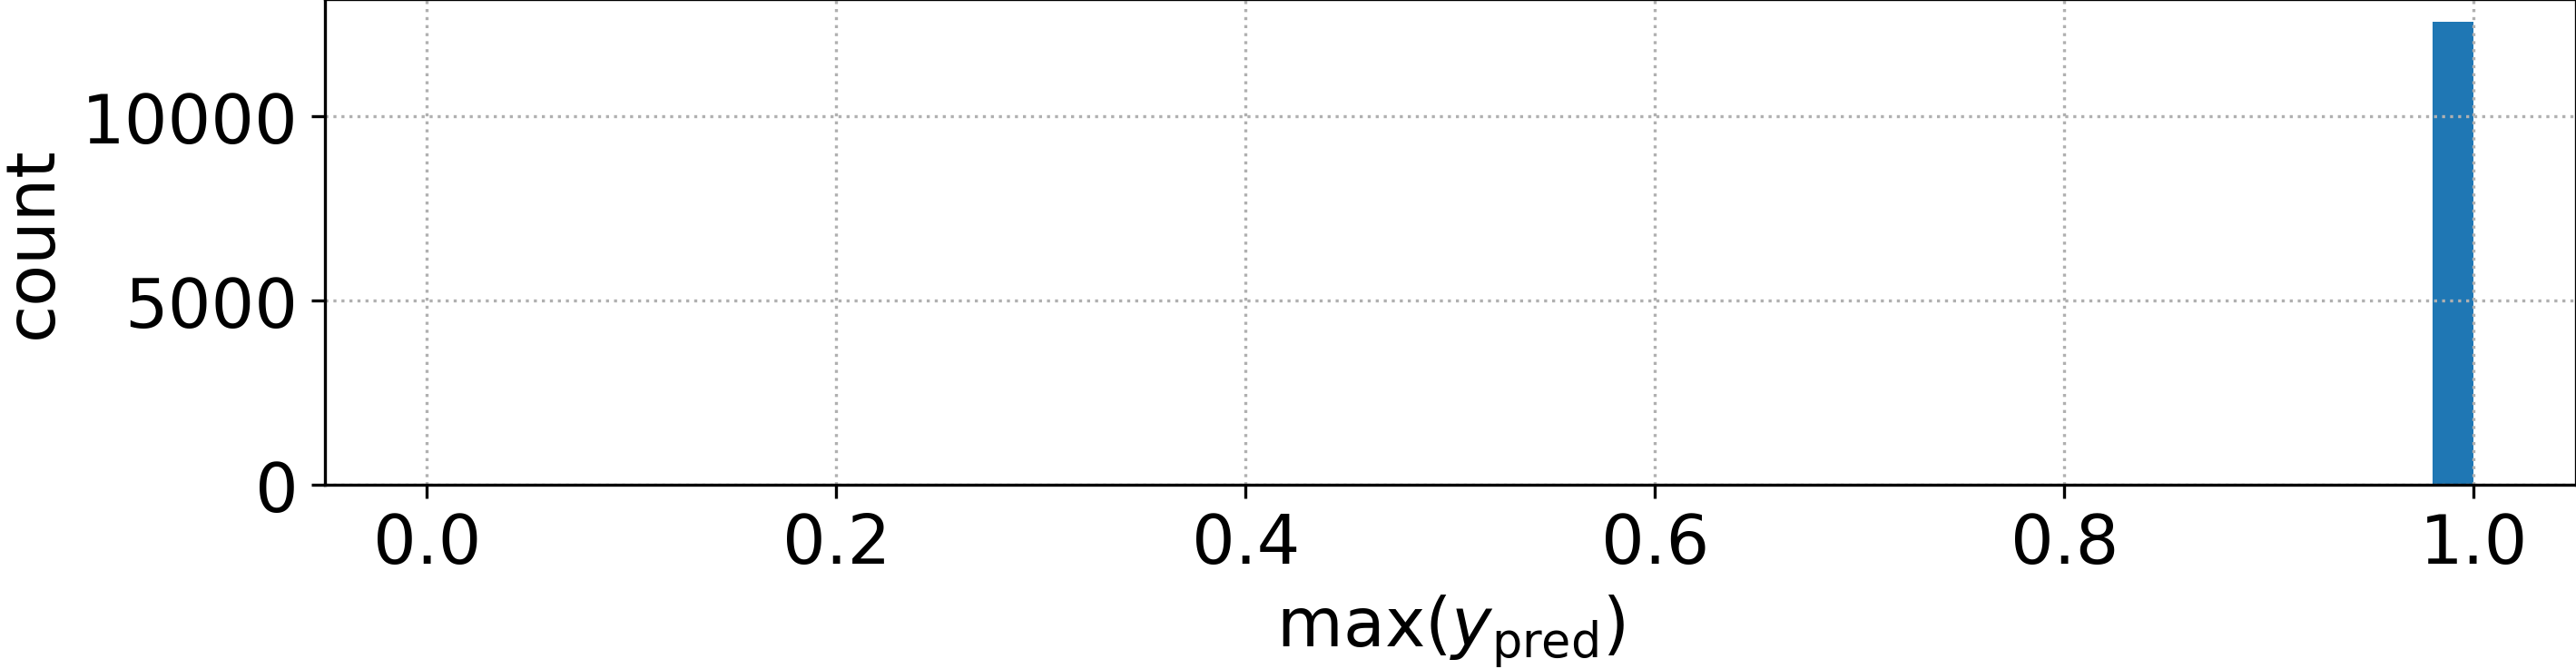
\includegraphics[width=0.6\textwidth]{figures/v2_real/vit_model_V2max_ypred_binary_26.png}
    \caption{Max value of the output vector from the Spectral ViT V2 Binary Classification.\label{fig:fig:v2_binary_pred}}
\end{figure}

% \begin{figure}[h]
%     \centering
%     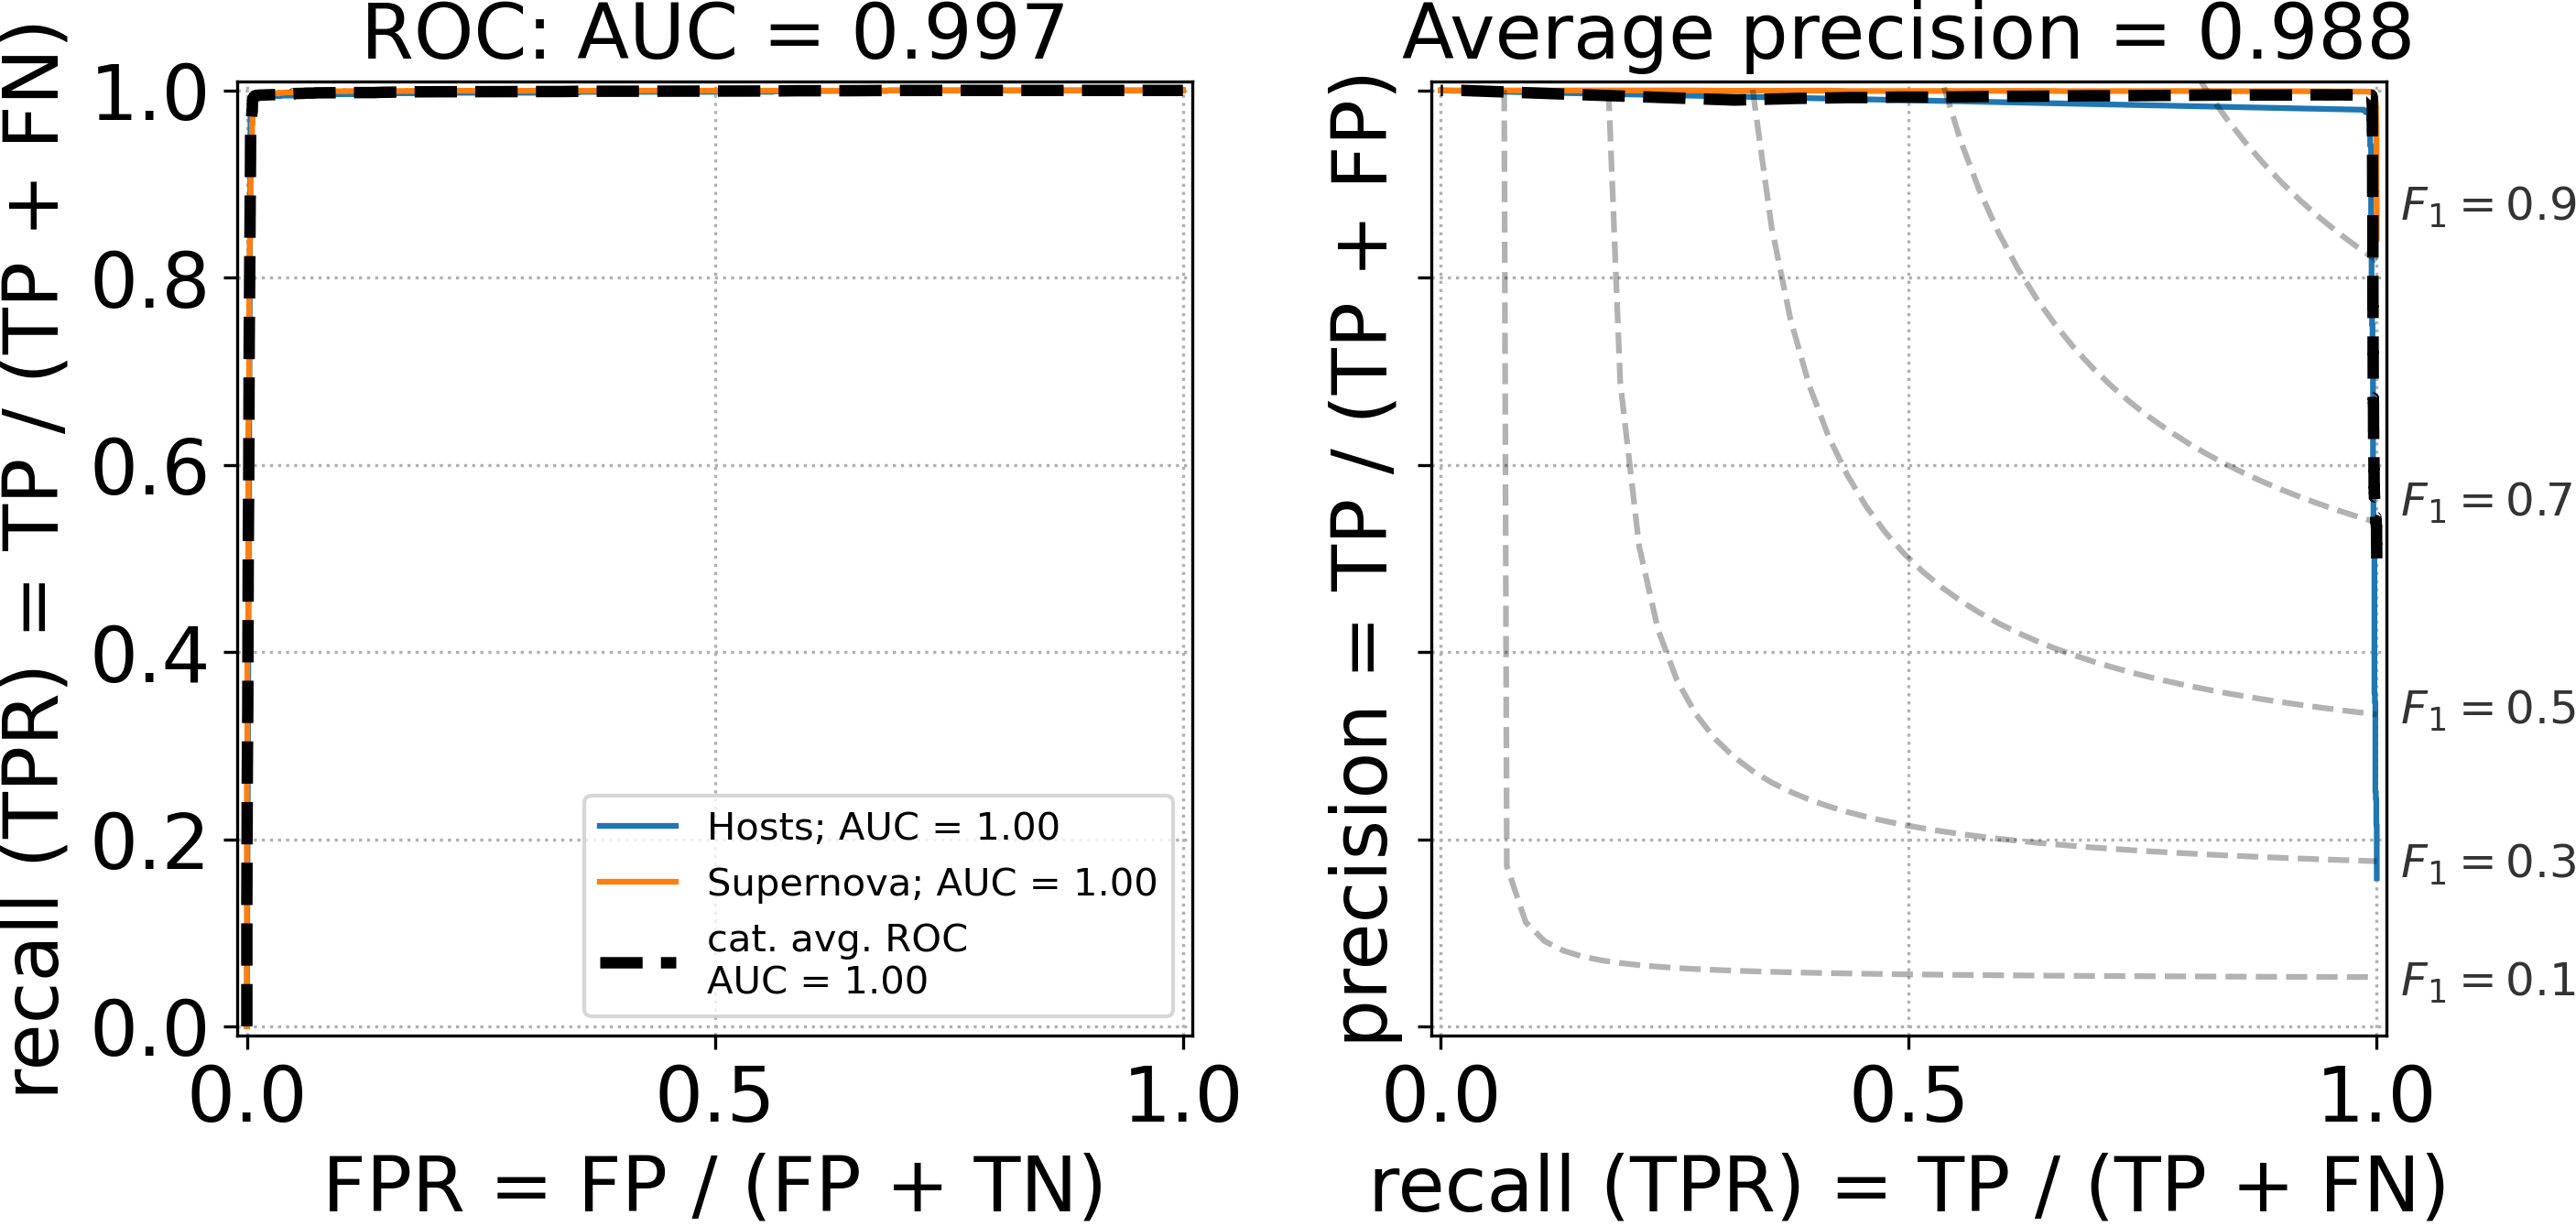
\includegraphics[height=4.2cm]{figures/v2_real/vit_model_V2roc9999_binary_e26.png}
%     \quad
%     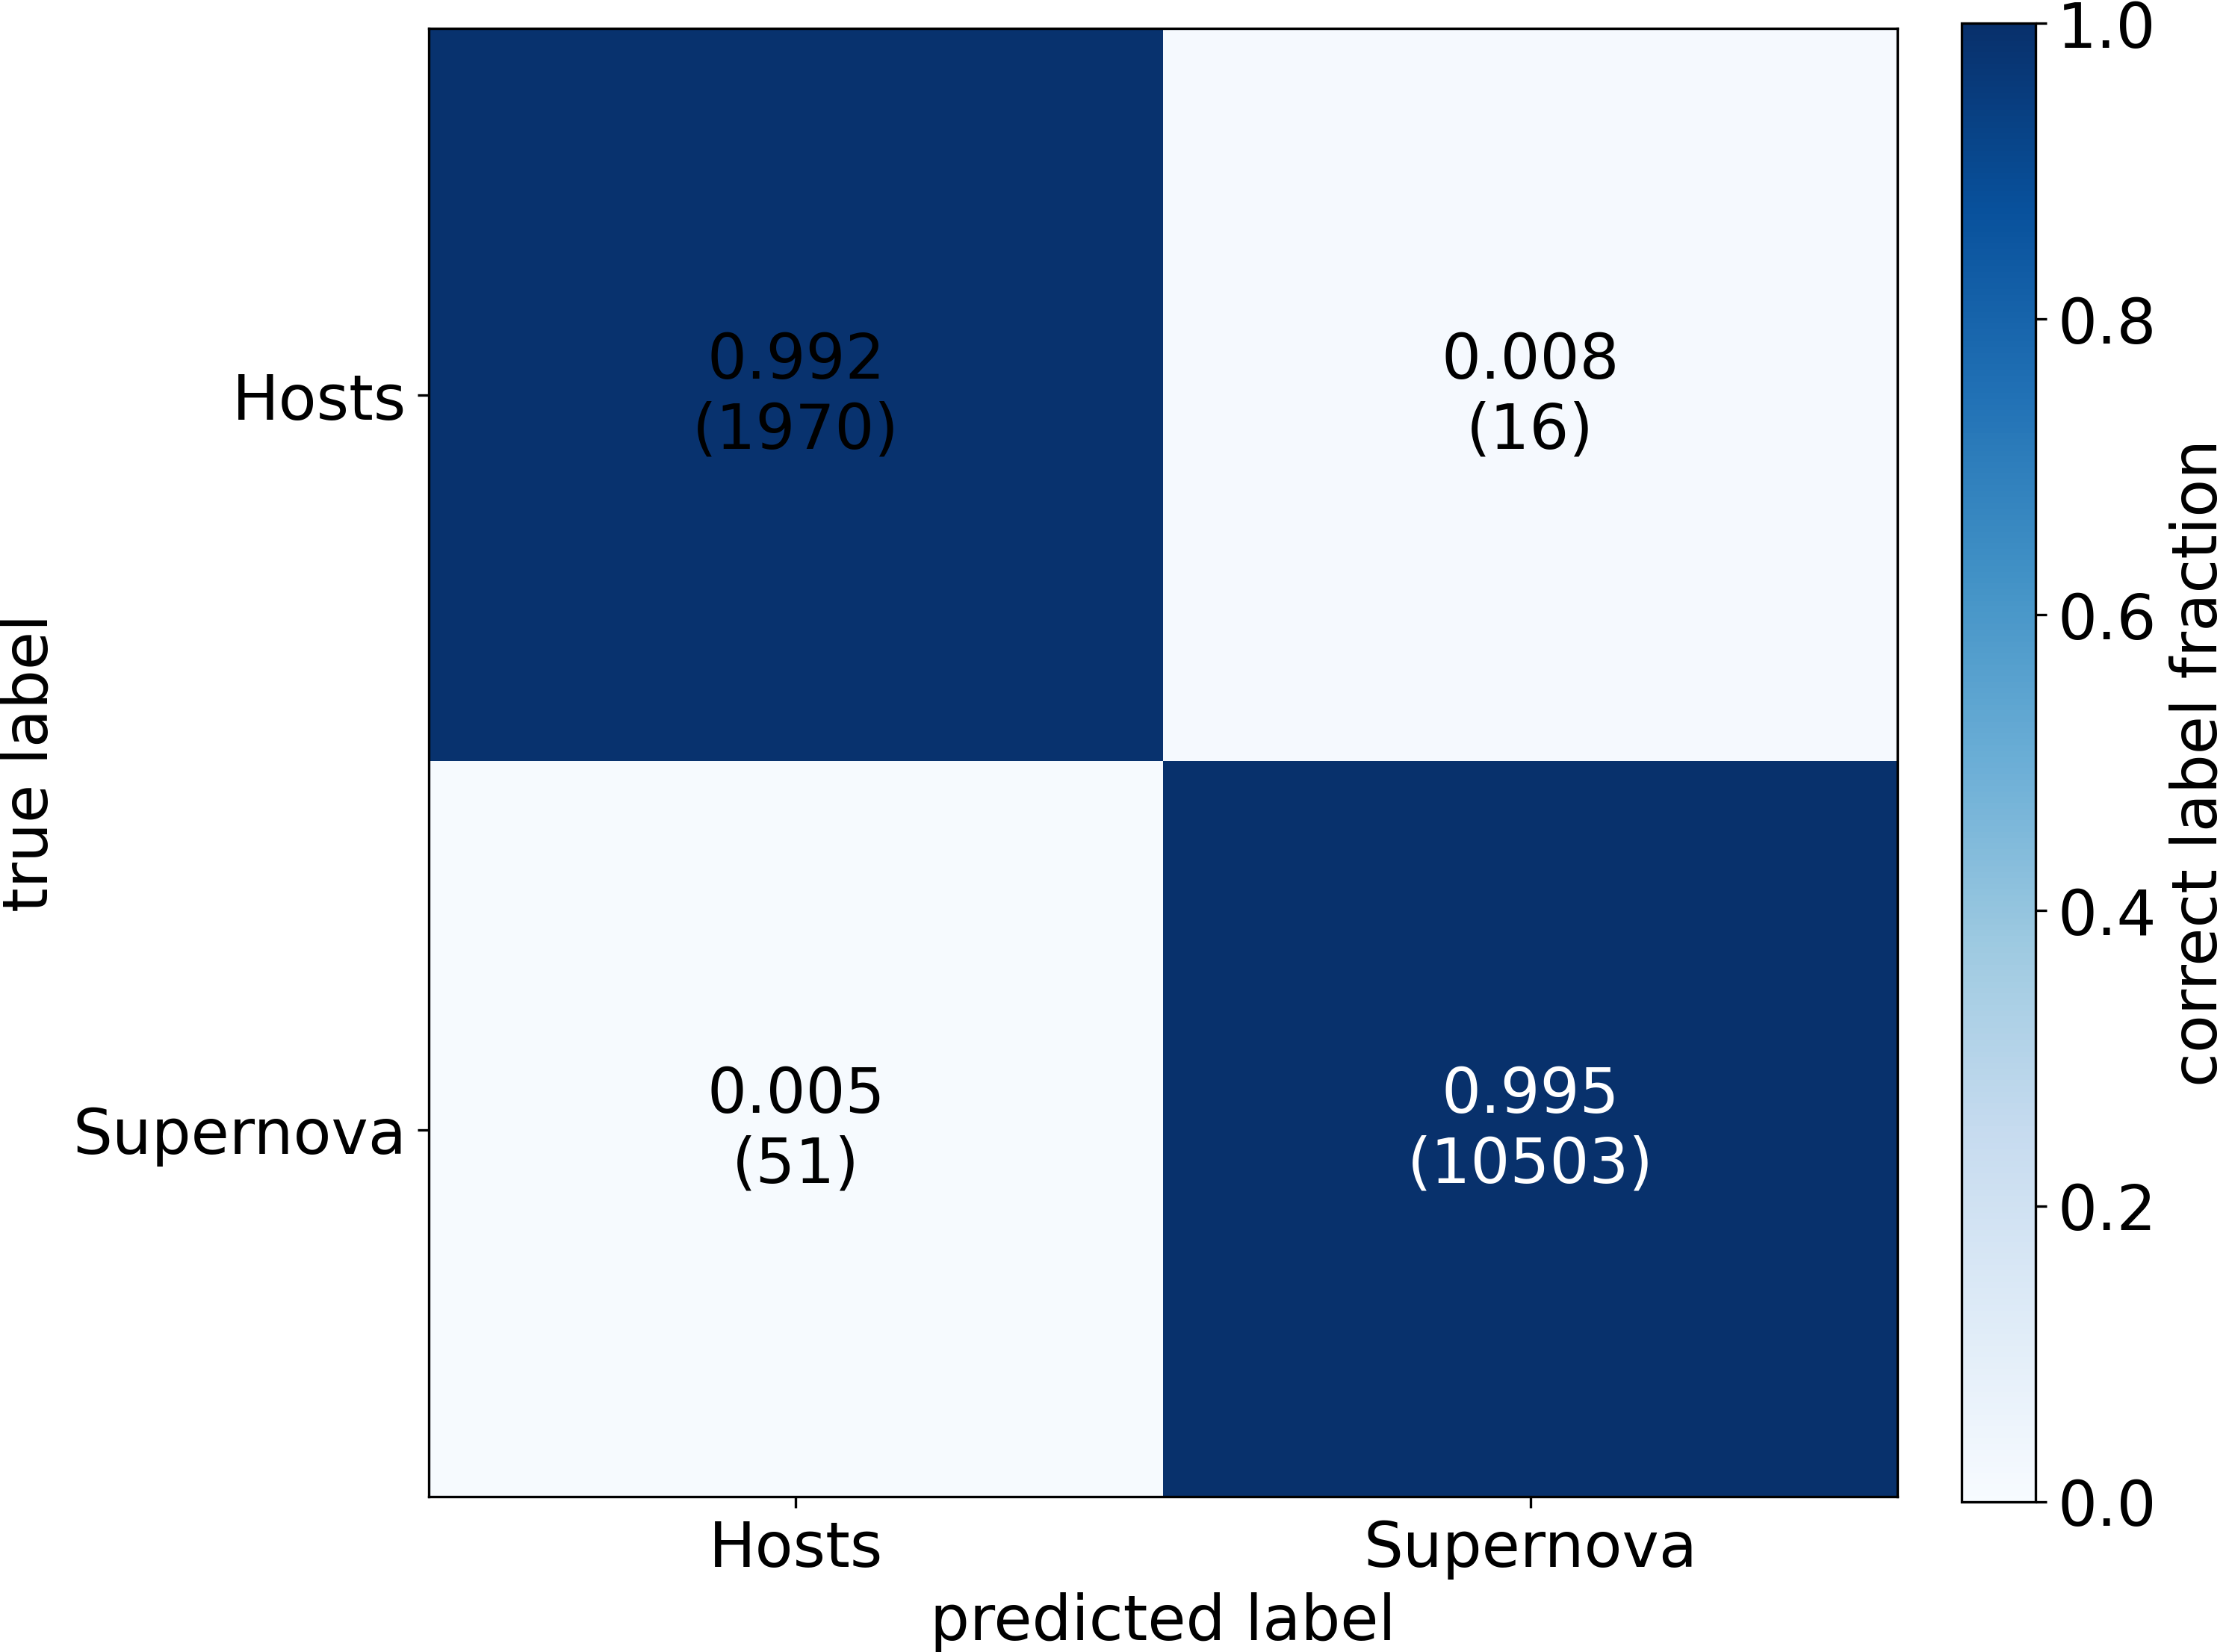
\includegraphics[height=4.2cm]{figures/v2_real/vit_model_V2cm9999_binary_e26.png}
%     \caption{Spectral ViT V2 Binary Diagnostics: ROC Curve (left) and Confusion Matrix (right) with a 99.99\% confidence
%     cut \label{fig:v2_binary_9999_qual}}
% \end{figure}

